% Options for packages loaded elsewhere
\PassOptionsToPackage{unicode}{hyperref}
\PassOptionsToPackage{hyphens}{url}
\PassOptionsToPackage{dvipsnames,svgnames,x11names}{xcolor}
%
\documentclass[
  letterpaper,
  DIV=11,
  numbers=noendperiod]{scrartcl}

\usepackage{amsmath,amssymb}
\usepackage{iftex}
\ifPDFTeX
  \usepackage[T1]{fontenc}
  \usepackage[utf8]{inputenc}
  \usepackage{textcomp} % provide euro and other symbols
\else % if luatex or xetex
  \usepackage{unicode-math}
  \defaultfontfeatures{Scale=MatchLowercase}
  \defaultfontfeatures[\rmfamily]{Ligatures=TeX,Scale=1}
\fi
\usepackage{lmodern}
\ifPDFTeX\else  
    % xetex/luatex font selection
\fi
% Use upquote if available, for straight quotes in verbatim environments
\IfFileExists{upquote.sty}{\usepackage{upquote}}{}
\IfFileExists{microtype.sty}{% use microtype if available
  \usepackage[]{microtype}
  \UseMicrotypeSet[protrusion]{basicmath} % disable protrusion for tt fonts
}{}
\makeatletter
\@ifundefined{KOMAClassName}{% if non-KOMA class
  \IfFileExists{parskip.sty}{%
    \usepackage{parskip}
  }{% else
    \setlength{\parindent}{0pt}
    \setlength{\parskip}{6pt plus 2pt minus 1pt}}
}{% if KOMA class
  \KOMAoptions{parskip=half}}
\makeatother
\usepackage{xcolor}
\setlength{\emergencystretch}{3em} % prevent overfull lines
\setcounter{secnumdepth}{5}
% Make \paragraph and \subparagraph free-standing
\ifx\paragraph\undefined\else
  \let\oldparagraph\paragraph
  \renewcommand{\paragraph}[1]{\oldparagraph{#1}\mbox{}}
\fi
\ifx\subparagraph\undefined\else
  \let\oldsubparagraph\subparagraph
  \renewcommand{\subparagraph}[1]{\oldsubparagraph{#1}\mbox{}}
\fi

\usepackage{color}
\usepackage{fancyvrb}
\newcommand{\VerbBar}{|}
\newcommand{\VERB}{\Verb[commandchars=\\\{\}]}
\DefineVerbatimEnvironment{Highlighting}{Verbatim}{commandchars=\\\{\}}
% Add ',fontsize=\small' for more characters per line
\usepackage{framed}
\definecolor{shadecolor}{RGB}{241,243,245}
\newenvironment{Shaded}{\begin{snugshade}}{\end{snugshade}}
\newcommand{\AlertTok}[1]{\textcolor[rgb]{0.68,0.00,0.00}{#1}}
\newcommand{\AnnotationTok}[1]{\textcolor[rgb]{0.37,0.37,0.37}{#1}}
\newcommand{\AttributeTok}[1]{\textcolor[rgb]{0.40,0.45,0.13}{#1}}
\newcommand{\BaseNTok}[1]{\textcolor[rgb]{0.68,0.00,0.00}{#1}}
\newcommand{\BuiltInTok}[1]{\textcolor[rgb]{0.00,0.23,0.31}{#1}}
\newcommand{\CharTok}[1]{\textcolor[rgb]{0.13,0.47,0.30}{#1}}
\newcommand{\CommentTok}[1]{\textcolor[rgb]{0.37,0.37,0.37}{#1}}
\newcommand{\CommentVarTok}[1]{\textcolor[rgb]{0.37,0.37,0.37}{\textit{#1}}}
\newcommand{\ConstantTok}[1]{\textcolor[rgb]{0.56,0.35,0.01}{#1}}
\newcommand{\ControlFlowTok}[1]{\textcolor[rgb]{0.00,0.23,0.31}{#1}}
\newcommand{\DataTypeTok}[1]{\textcolor[rgb]{0.68,0.00,0.00}{#1}}
\newcommand{\DecValTok}[1]{\textcolor[rgb]{0.68,0.00,0.00}{#1}}
\newcommand{\DocumentationTok}[1]{\textcolor[rgb]{0.37,0.37,0.37}{\textit{#1}}}
\newcommand{\ErrorTok}[1]{\textcolor[rgb]{0.68,0.00,0.00}{#1}}
\newcommand{\ExtensionTok}[1]{\textcolor[rgb]{0.00,0.23,0.31}{#1}}
\newcommand{\FloatTok}[1]{\textcolor[rgb]{0.68,0.00,0.00}{#1}}
\newcommand{\FunctionTok}[1]{\textcolor[rgb]{0.28,0.35,0.67}{#1}}
\newcommand{\ImportTok}[1]{\textcolor[rgb]{0.00,0.46,0.62}{#1}}
\newcommand{\InformationTok}[1]{\textcolor[rgb]{0.37,0.37,0.37}{#1}}
\newcommand{\KeywordTok}[1]{\textcolor[rgb]{0.00,0.23,0.31}{#1}}
\newcommand{\NormalTok}[1]{\textcolor[rgb]{0.00,0.23,0.31}{#1}}
\newcommand{\OperatorTok}[1]{\textcolor[rgb]{0.37,0.37,0.37}{#1}}
\newcommand{\OtherTok}[1]{\textcolor[rgb]{0.00,0.23,0.31}{#1}}
\newcommand{\PreprocessorTok}[1]{\textcolor[rgb]{0.68,0.00,0.00}{#1}}
\newcommand{\RegionMarkerTok}[1]{\textcolor[rgb]{0.00,0.23,0.31}{#1}}
\newcommand{\SpecialCharTok}[1]{\textcolor[rgb]{0.37,0.37,0.37}{#1}}
\newcommand{\SpecialStringTok}[1]{\textcolor[rgb]{0.13,0.47,0.30}{#1}}
\newcommand{\StringTok}[1]{\textcolor[rgb]{0.13,0.47,0.30}{#1}}
\newcommand{\VariableTok}[1]{\textcolor[rgb]{0.07,0.07,0.07}{#1}}
\newcommand{\VerbatimStringTok}[1]{\textcolor[rgb]{0.13,0.47,0.30}{#1}}
\newcommand{\WarningTok}[1]{\textcolor[rgb]{0.37,0.37,0.37}{\textit{#1}}}

\providecommand{\tightlist}{%
  \setlength{\itemsep}{0pt}\setlength{\parskip}{0pt}}\usepackage{longtable,booktabs,array}
\usepackage{calc} % for calculating minipage widths
% Correct order of tables after \paragraph or \subparagraph
\usepackage{etoolbox}
\makeatletter
\patchcmd\longtable{\par}{\if@noskipsec\mbox{}\fi\par}{}{}
\makeatother
% Allow footnotes in longtable head/foot
\IfFileExists{footnotehyper.sty}{\usepackage{footnotehyper}}{\usepackage{footnote}}
\makesavenoteenv{longtable}
\usepackage{graphicx}
\makeatletter
\def\maxwidth{\ifdim\Gin@nat@width>\linewidth\linewidth\else\Gin@nat@width\fi}
\def\maxheight{\ifdim\Gin@nat@height>\textheight\textheight\else\Gin@nat@height\fi}
\makeatother
% Scale images if necessary, so that they will not overflow the page
% margins by default, and it is still possible to overwrite the defaults
% using explicit options in \includegraphics[width, height, ...]{}
\setkeys{Gin}{width=\maxwidth,height=\maxheight,keepaspectratio}
% Set default figure placement to htbp
\makeatletter
\def\fps@figure{htbp}
\makeatother

\KOMAoption{captions}{tableheading}
\makeatletter
\makeatother
\makeatletter
\makeatother
\makeatletter
\@ifpackageloaded{caption}{}{\usepackage{caption}}
\AtBeginDocument{%
\ifdefined\contentsname
  \renewcommand*\contentsname{Table of contents}
\else
  \newcommand\contentsname{Table of contents}
\fi
\ifdefined\listfigurename
  \renewcommand*\listfigurename{List of Figures}
\else
  \newcommand\listfigurename{List of Figures}
\fi
\ifdefined\listtablename
  \renewcommand*\listtablename{List of Tables}
\else
  \newcommand\listtablename{List of Tables}
\fi
\ifdefined\figurename
  \renewcommand*\figurename{Figure}
\else
  \newcommand\figurename{Figure}
\fi
\ifdefined\tablename
  \renewcommand*\tablename{Table}
\else
  \newcommand\tablename{Table}
\fi
}
\@ifpackageloaded{float}{}{\usepackage{float}}
\floatstyle{ruled}
\@ifundefined{c@chapter}{\newfloat{codelisting}{h}{lop}}{\newfloat{codelisting}{h}{lop}[chapter]}
\floatname{codelisting}{Stan Program}
\newcommand*\listoflistings{\listof{codelisting}{List of Listings}}
\makeatother
\makeatletter
\@ifpackageloaded{caption}{}{\usepackage{caption}}
\@ifpackageloaded{subcaption}{}{\usepackage{subcaption}}
\makeatother
\makeatletter
\@ifpackageloaded{tcolorbox}{}{\usepackage[skins,breakable]{tcolorbox}}
\makeatother
\makeatletter
\@ifundefined{shadecolor}{\definecolor{shadecolor}{rgb}{.97, .97, .97}}
\makeatother
\makeatletter
\makeatother
\makeatletter
\makeatother
\ifLuaTeX
  \usepackage{selnolig}  % disable illegal ligatures
\fi
\IfFileExists{bookmark.sty}{\usepackage{bookmark}}{\usepackage{hyperref}}
\IfFileExists{xurl.sty}{\usepackage{xurl}}{} % add URL line breaks if available
\urlstyle{same} % disable monospaced font for URLs
\hypersetup{
  pdftitle={Modeling Tree Diameter Growth},
  pdfauthor={Michael Betancourt},
  colorlinks=true,
  linkcolor={blue},
  filecolor={Maroon},
  citecolor={Blue},
  urlcolor={Blue},
  pdfcreator={LaTeX via pandoc}}

\title{Modeling Tree Diameter Growth}
\author{Michael Betancourt}
\date{January 2024}

\begin{document}
\maketitle
\ifdefined\Shaded\renewenvironment{Shaded}{\begin{tcolorbox}[boxrule=0pt, sharp corners, interior hidden, breakable, borderline west={3pt}{0pt}{shadecolor}, enhanced, frame hidden]}{\end{tcolorbox}}\fi

\renewcommand*\contentsname{Table of contents}
{
\hypersetup{linkcolor=}
\setcounter{tocdepth}{3}
\tableofcontents
}
Because tree growth is sensitive to the surrounding environmental, in
particular the ambient climate, continual measurements of tree growth
are a powerful way to learn about the history of changes to that
environment. In this exercise we'll explore a Bayesian approach to
modeling and drawing inferences from tree diameter data measurements,
with a focus on capturing the underlying data generating process. At the
end I'll discuss how this exercise was integrated into a two-day
interactive workshop.

\hypertarget{familiarizing-ourselves-with-the-data}{%
\section{Familiarizing Ourselves With The
Data}\label{familiarizing-ourselves-with-the-data}}

Before building any models we need to understand is being modeled. In
particular we need to develop our understanding of the data and its
provenance.

\hypertarget{sec:provenance}{%
\subsection{Data Provenance}\label{sec:provenance}}

The data with which we'll be working consists of \textbf{diameter at
breast height}, or \textbf{DBH}, measurements. These measurements are
made by wrapping a measuring tape around the trunk of a tree at a height
of 1.37 meters, approximating the breast height of an average human
(Figure~\ref{fig-diameter-measurement}). This height is high enough to
avoid the tree roots and forest floor but low enough to be accessible to
researchers making the measurements. Diameter observations are given by
dividing the recorded circumference by \(\pi\).

When the diameter of a tree is first measured it is marked with a tag to
indicate the breast height used. All future diameter measurements are
made at the tag height to ensure consistency across time.

\begin{figure}

{\centering 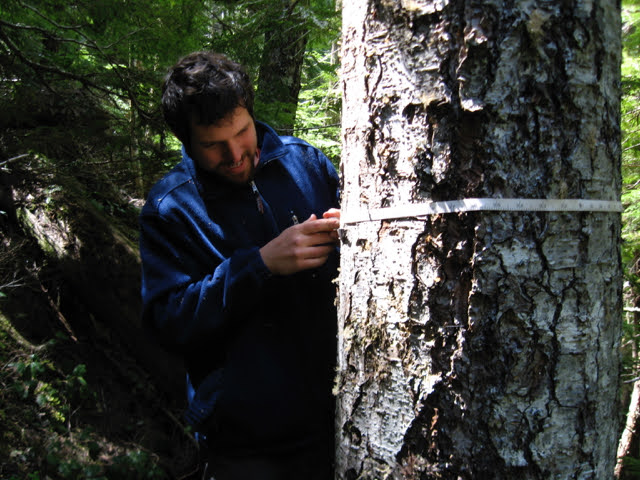
\includegraphics[width=0.5\textwidth,height=\textheight]{figures/photos/diameter_measurement_ii.jpg}

}

\caption{\label{fig-diameter-measurement}Tree diameters are measured by
wrapping a measuring tape around the trunk of a tree 1.37 meters above
the ground and then dividing the recorded circumference by \(\pi\). Here
Robert Ettinger is recording tree diameters in the Pacific Northwest.
Photo :copyright: Ailene Ettinger, used with permission.}

\end{figure}

The H.J. Andrews Experimental Forest and Long Term Ecological Research
Program has censused trees in forests across the Pacific Northwest every
five or six years for decades. In addition to the tree diameter
additional physiological attributes, such as tree vigor and the
condition of the tree crown and stem are also recorded. If a tree is
found to have died since it was last measured then a mortality
assessment is also performed. For intimate detail on the measurement
procedures and the structure of the resulting data see the
\href{https://github.com/lizzieinvancouver/bayesian2024ubc/tree/main/data/treestands/metadata/PSP_tree_measurement_protocol_v2019.pdf}{Pacific
Northwest Permanent Sample Plot Program Protocol for Tree Measurements
and Mortality Assessments}.

In this exercise we will be focusing on data collected from forests
around Mount Rainier (Figure~\ref{fig-mount-rainier}). These forests
cover a wide range of elevations and other environmental conditions
which make them particularly well-suited for studying various aspects of
an evolving climate. That said here we will consider only trees that are
isolated to a single stand of forest.

\begin{figure}

{\centering 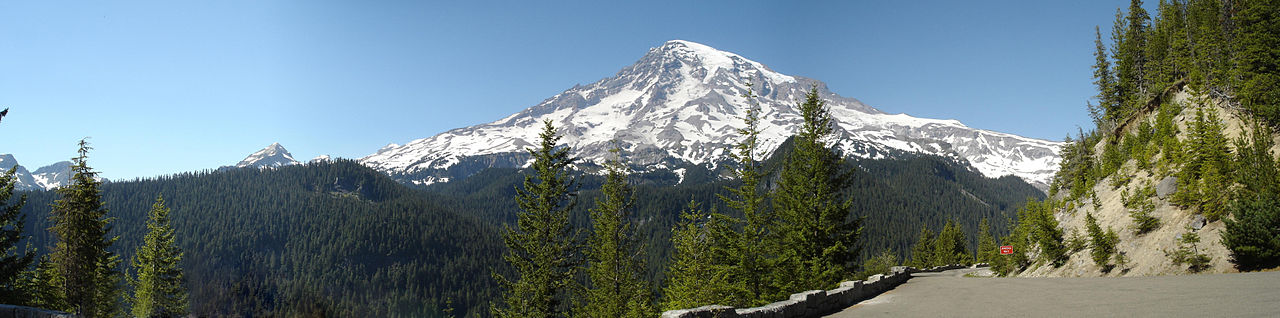
\includegraphics[width=1\textwidth,height=\textheight]{figures/photos/mount_rainier_panorama.jpg}

}

\caption{\label{fig-mount-rainier}The forests around Mount Rainier span
a diversity of environmental conditions. Photo courtesy of WikiMedia,
\url{https://commons.wikimedia.org/wiki/File:Mount_Rainier_panorama_2.jpg}.}

\end{figure}

\hypertarget{sec:initial-setup}{%
\subsection{Code Environment Set Up}\label{sec:initial-setup}}

With the provenance established we're ready to take our first peak at
the data itself. We'll start by configuring our local \texttt{R}
environment for some reasonably aesthetic visualizations.

\begin{Shaded}
\begin{Highlighting}[]
\FunctionTok{par}\NormalTok{(}\AttributeTok{family=}\StringTok{"serif"}\NormalTok{, }\AttributeTok{las=}\DecValTok{1}\NormalTok{, }\AttributeTok{bty=}\StringTok{"l"}\NormalTok{,}
    \AttributeTok{cex.axis=}\DecValTok{1}\NormalTok{, }\AttributeTok{cex.lab=}\DecValTok{1}\NormalTok{, }\AttributeTok{cex.main=}\DecValTok{1}\NormalTok{,}
    \AttributeTok{xaxs=}\StringTok{"i"}\NormalTok{, }\AttributeTok{yaxs=}\StringTok{"i"}\NormalTok{, }\AttributeTok{mar =} \FunctionTok{c}\NormalTok{(}\DecValTok{5}\NormalTok{, }\DecValTok{5}\NormalTok{, }\DecValTok{3}\NormalTok{, }\DecValTok{5}\NormalTok{))}

\NormalTok{c\_light }\OtherTok{\textless{}{-}} \FunctionTok{c}\NormalTok{(}\StringTok{"\#DCBCBC"}\NormalTok{)}
\NormalTok{c\_light\_highlight }\OtherTok{\textless{}{-}} \FunctionTok{c}\NormalTok{(}\StringTok{"\#C79999"}\NormalTok{)}
\NormalTok{c\_mid }\OtherTok{\textless{}{-}} \FunctionTok{c}\NormalTok{(}\StringTok{"\#B97C7C"}\NormalTok{)}
\NormalTok{c\_mid\_highlight }\OtherTok{\textless{}{-}} \FunctionTok{c}\NormalTok{(}\StringTok{"\#A25050"}\NormalTok{)}
\NormalTok{c\_dark }\OtherTok{\textless{}{-}} \FunctionTok{c}\NormalTok{(}\StringTok{"\#8F2727"}\NormalTok{)}
\NormalTok{c\_dark\_highlight }\OtherTok{\textless{}{-}} \FunctionTok{c}\NormalTok{(}\StringTok{"\#7C0000"}\NormalTok{)}

\NormalTok{c\_light\_teal }\OtherTok{\textless{}{-}} \FunctionTok{c}\NormalTok{(}\StringTok{"\#6B8E8E"}\NormalTok{)}
\NormalTok{c\_mid\_teal }\OtherTok{\textless{}{-}} \FunctionTok{c}\NormalTok{(}\StringTok{"\#487575"}\NormalTok{)}
\NormalTok{c\_dark\_teal }\OtherTok{\textless{}{-}} \FunctionTok{c}\NormalTok{(}\StringTok{"\#1D4F4F"}\NormalTok{)}
\end{Highlighting}
\end{Shaded}

\hypertarget{sec:eda}{%
\subsection{Exploratory Data Analysis}\label{sec:eda}}

We now read in our data for stand AV06. The columns and their possible
values are carefully documented in
\href{https://github.com/lizzieinvancouver/bayesian2024ubc/tree/main/data/treestands/metadata/PSP_tree_measurement_protocol_v2019.pdf}{Pacific
Northwest Permanent Sample Plot Program Protocol for Tree Measurements
and Mortality Assessments}.

\begin{Shaded}
\begin{Highlighting}[]
\NormalTok{stand\_tree\_data }\OtherTok{\textless{}{-}} \FunctionTok{read.csv}\NormalTok{(}\StringTok{\textquotesingle{}data/TV01002\_v17\_AV06.csv\textquotesingle{}}\NormalTok{, }\AttributeTok{skip=}\DecValTok{5}\NormalTok{)}
\end{Highlighting}
\end{Shaded}

To ensure that visualizations fit nicely into this document I'm going to
restrict consideration to only the first 22 trees in the stand.

\begin{Shaded}
\begin{Highlighting}[]
\NormalTok{tree\_ids }\OtherTok{\textless{}{-}}  \FunctionTok{unique}\NormalTok{(stand\_tree\_data}\SpecialCharTok{$}\NormalTok{TREEID)}

\NormalTok{N\_trees }\OtherTok{\textless{}{-}} \DecValTok{22}
\NormalTok{tree\_ids }\OtherTok{\textless{}{-}}\NormalTok{ tree\_ids[}\DecValTok{1}\SpecialCharTok{:}\NormalTok{N\_trees]}
\end{Highlighting}
\end{Shaded}

In this nominal format repeated measurements of a given tree are not
necessarily organized next to each other. Because we are particularly
interested in tree diameter growth it will be much more convenient to
collect repeated measurements together and construct indices that allow
us to readily isolate the data for a single tree.

Note how we're using our understanding of the data generating process to
motivate how we format and visualize the data. Exploratory data analysis
is always done in the context of as assumed, if conceptual, data
generating process!

\begin{Shaded}
\begin{Highlighting}[]
\NormalTok{tree\_N\_obs }\OtherTok{\textless{}{-}} \FunctionTok{c}\NormalTok{()}
\NormalTok{tree\_start\_idxs }\OtherTok{\textless{}{-}} \FunctionTok{c}\NormalTok{()}
\NormalTok{tree\_end\_idxs }\OtherTok{\textless{}{-}} \FunctionTok{c}\NormalTok{()}
\NormalTok{tree\_years }\OtherTok{\textless{}{-}} \FunctionTok{c}\NormalTok{()}
\NormalTok{tree\_dbhs }\OtherTok{\textless{}{-}} \FunctionTok{c}\NormalTok{()}
\NormalTok{tree\_vigors }\OtherTok{\textless{}{-}} \FunctionTok{c}\NormalTok{()}
\NormalTok{tree\_species }\OtherTok{\textless{}{-}} \FunctionTok{c}\NormalTok{()}
\NormalTok{tree\_statuses }\OtherTok{\textless{}{-}} \FunctionTok{c}\NormalTok{()}
\NormalTok{tree\_notes }\OtherTok{\textless{}{-}} \FunctionTok{c}\NormalTok{()}

\NormalTok{idx }\OtherTok{\textless{}{-}} \DecValTok{1}

\ControlFlowTok{for}\NormalTok{ (id }\ControlFlowTok{in}\NormalTok{ tree\_ids) \{}
  \CommentTok{\# Isolate observations for given tree}
\NormalTok{  tree\_data }\OtherTok{\textless{}{-}}\NormalTok{ stand\_tree\_data[stand\_tree\_data[}\StringTok{\textquotesingle{}TREEID\textquotesingle{}}\NormalTok{] }\SpecialCharTok{==}\NormalTok{ id,]}

\NormalTok{  years }\OtherTok{\textless{}{-}}\NormalTok{ tree\_data[,}\StringTok{\textquotesingle{}YEAR\textquotesingle{}}\NormalTok{]}
\NormalTok{  dbhs }\OtherTok{\textless{}{-}}\NormalTok{ tree\_data[,}\StringTok{\textquotesingle{}DBH\textquotesingle{}}\NormalTok{]}
\NormalTok{  vigors }\OtherTok{\textless{}{-}}\NormalTok{ tree\_data[,}\StringTok{\textquotesingle{}TREE\_VIGOR\textquotesingle{}}\NormalTok{]}
\NormalTok{  species }\OtherTok{\textless{}{-}}\NormalTok{ tree\_data[,}\StringTok{\textquotesingle{}SPECIES\textquotesingle{}}\NormalTok{]}
\NormalTok{  statuses }\OtherTok{\textless{}{-}}\NormalTok{ tree\_data[,}\StringTok{\textquotesingle{}TREE\_STATUS\textquotesingle{}}\NormalTok{]}
\NormalTok{  notes }\OtherTok{\textless{}{-}}\NormalTok{ tree\_data[,}\StringTok{\textquotesingle{}CHECK\_NOTES\textquotesingle{}}\NormalTok{]}

  \CommentTok{\# Append tree data}
\NormalTok{  N\_obs }\OtherTok{\textless{}{-}} \FunctionTok{length}\NormalTok{(years)}
\NormalTok{  tree\_N\_obs }\OtherTok{\textless{}{-}} \FunctionTok{c}\NormalTok{(tree\_N\_obs, N\_obs)}

\NormalTok{  start\_idx }\OtherTok{\textless{}{-}}\NormalTok{ idx}
\NormalTok{  end\_idx }\OtherTok{\textless{}{-}}\NormalTok{ idx }\SpecialCharTok{+}\NormalTok{ N\_obs }\SpecialCharTok{{-}} \DecValTok{1}
\NormalTok{  idx }\OtherTok{\textless{}{-}}\NormalTok{ idx }\SpecialCharTok{+}\NormalTok{ N\_obs}
\NormalTok{  tree\_start\_idxs }\OtherTok{\textless{}{-}} \FunctionTok{c}\NormalTok{(tree\_start\_idxs, start\_idx)}
\NormalTok{  tree\_end\_idxs }\OtherTok{\textless{}{-}} \FunctionTok{c}\NormalTok{(tree\_end\_idxs, end\_idx)}

\NormalTok{  tree\_years }\OtherTok{\textless{}{-}} \FunctionTok{c}\NormalTok{(tree\_years, years)}
\NormalTok{  tree\_dbhs }\OtherTok{\textless{}{-}} \FunctionTok{c}\NormalTok{(tree\_dbhs, dbhs)}
\NormalTok{  tree\_species }\OtherTok{\textless{}{-}} \FunctionTok{c}\NormalTok{(tree\_species, species)}
\NormalTok{  tree\_vigors }\OtherTok{\textless{}{-}} \FunctionTok{c}\NormalTok{(tree\_vigors, vigors)}
\NormalTok{  tree\_statuses }\OtherTok{\textless{}{-}} \FunctionTok{c}\NormalTok{(tree\_statuses, statuses)}
\NormalTok{  tree\_notes }\OtherTok{\textless{}{-}} \FunctionTok{c}\NormalTok{(tree\_notes, notes)}
\NormalTok{\}}
\end{Highlighting}
\end{Shaded}

Each tree diameter measurement is accompanied by many different
assessments of the tree's condition. For our initial investigation I
take a look at \textbf{tree vigor} which is a general quantification of
health. We can communicate tree vigor in our visualizations by coloring
each observation according to the five possible statuses.

\begin{Shaded}
\begin{Highlighting}[]
\NormalTok{vigor\_cols }\OtherTok{\textless{}{-}} \FunctionTok{list}\NormalTok{(}\StringTok{"1"} \OtherTok{=}\NormalTok{ c\_dark, }\StringTok{"2"} \OtherTok{=}\NormalTok{ c\_mid, }\StringTok{"3"} \OtherTok{=}\NormalTok{ c\_light,}
                   \StringTok{"U"} \OtherTok{=}\NormalTok{ c\_mid\_teal, }\StringTok{"M"} \OtherTok{=} \StringTok{"black"}\NormalTok{)}
\end{Highlighting}
\end{Shaded}

This reorganization of the data makes it straightforward to plot a time
series of measurements for each tree. Each observation is colored
according to the tree vigor. Observations of dead trees with
\texttt{TREE\_VIGOR\ =\ "M"} are given \texttt{NA} diameters values;
these will be denoted with gray rectangles at the corresponding
observation year.

\begin{Shaded}
\begin{Highlighting}[]
\NormalTok{plot\_tree\_data }\OtherTok{\textless{}{-}} \ControlFlowTok{function}\NormalTok{(t) \{}
\NormalTok{  tree\_idxs }\OtherTok{\textless{}{-}}\NormalTok{ tree\_start\_idxs[t]}\SpecialCharTok{:}\NormalTok{tree\_end\_idxs[t]}

\NormalTok{  years }\OtherTok{\textless{}{-}}\NormalTok{ tree\_years[tree\_idxs]}
\NormalTok{  dbhs }\OtherTok{\textless{}{-}}\NormalTok{ tree\_dbhs[tree\_idxs]}
\NormalTok{  vigors }\OtherTok{\textless{}{-}}\NormalTok{ tree\_vigors[tree\_idxs]}
\NormalTok{  cols }\OtherTok{=} \FunctionTok{sapply}\NormalTok{(vigors, }\ControlFlowTok{function}\NormalTok{(v) vigor\_cols[[v]])}

\NormalTok{  xlims }\OtherTok{\textless{}{-}} \FunctionTok{range}\NormalTok{(years)}
\NormalTok{  delta }\OtherTok{\textless{}{-}}\NormalTok{ xlims[}\DecValTok{2}\NormalTok{] }\SpecialCharTok{{-}}\NormalTok{ xlims[}\DecValTok{1}\NormalTok{]}
\NormalTok{  xlims[}\DecValTok{1}\NormalTok{] }\OtherTok{\textless{}{-}}\NormalTok{ xlims[}\DecValTok{1}\NormalTok{] }\SpecialCharTok{{-}} \FloatTok{0.1} \SpecialCharTok{*}\NormalTok{ delta}
\NormalTok{  xlims[}\DecValTok{2}\NormalTok{] }\OtherTok{\textless{}{-}}\NormalTok{ xlims[}\DecValTok{2}\NormalTok{] }\SpecialCharTok{+} \FloatTok{0.1} \SpecialCharTok{*}\NormalTok{ delta}

\NormalTok{  ylims }\OtherTok{\textless{}{-}} \FunctionTok{range}\NormalTok{(dbhs, }\AttributeTok{na.rm=}\ConstantTok{TRUE}\NormalTok{)}
\NormalTok{  delta }\OtherTok{\textless{}{-}}\NormalTok{ ylims[}\DecValTok{2}\NormalTok{] }\SpecialCharTok{{-}}\NormalTok{ ylims[}\DecValTok{1}\NormalTok{]}
\NormalTok{  ylims[}\DecValTok{1}\NormalTok{] }\OtherTok{\textless{}{-}}\NormalTok{ ylims[}\DecValTok{1}\NormalTok{] }\SpecialCharTok{{-}} \FloatTok{0.1} \SpecialCharTok{*}\NormalTok{ delta}
\NormalTok{  ylims[}\DecValTok{2}\NormalTok{] }\OtherTok{\textless{}{-}}\NormalTok{ ylims[}\DecValTok{2}\NormalTok{] }\SpecialCharTok{+} \FloatTok{0.1} \SpecialCharTok{*}\NormalTok{ delta}

  \FunctionTok{plot}\NormalTok{(years, dbhs,}
       \AttributeTok{main=}\FunctionTok{paste0}\NormalTok{(tree\_ids[t], }\StringTok{"}\SpecialCharTok{\textbackslash{}n}\StringTok{Local Tree Index = "}\NormalTok{, t),}
       \AttributeTok{pch=}\DecValTok{16}\NormalTok{, }\AttributeTok{cex=}\FloatTok{0.8}\NormalTok{, }\AttributeTok{col=}\NormalTok{cols,}
       \AttributeTok{xlab=}\StringTok{"Year"}\NormalTok{, }\AttributeTok{xlim=}\NormalTok{xlims, }\AttributeTok{ylab=}\StringTok{"DBH"}\NormalTok{, }\AttributeTok{ylim=}\NormalTok{ylims)}

\NormalTok{  na\_idxs }\OtherTok{\textless{}{-}} \FunctionTok{which}\NormalTok{(}\FunctionTok{is.na}\NormalTok{(dbhs))}
  \ControlFlowTok{for}\NormalTok{ (na\_idx }\ControlFlowTok{in}\NormalTok{ na\_idxs) \{}
    \FunctionTok{abline}\NormalTok{(}\AttributeTok{v=}\NormalTok{years[na\_idx], }\AttributeTok{col=}\StringTok{\textquotesingle{}\#DDDDDD\textquotesingle{}}\NormalTok{, }\AttributeTok{lwd=}\DecValTok{3}\NormalTok{)}
\NormalTok{  \}}
\NormalTok{\}}
\end{Highlighting}
\end{Shaded}

So how does our data look?

\begin{Shaded}
\begin{Highlighting}[]
\FunctionTok{par}\NormalTok{(}\AttributeTok{mfrow=}\FunctionTok{c}\NormalTok{(}\DecValTok{3}\NormalTok{, }\DecValTok{3}\NormalTok{))}
\ControlFlowTok{for}\NormalTok{ (t }\ControlFlowTok{in} \DecValTok{1}\SpecialCharTok{:}\DecValTok{18}\NormalTok{) \{}
  \FunctionTok{plot\_tree\_data}\NormalTok{(t)}
\NormalTok{\}}
\end{Highlighting}
\end{Shaded}

\begin{figure}[H]

{\centering \includegraphics{tree_diameter_growth_analysis_files/figure-pdf/unnamed-chunk-8-1.pdf}

}

\end{figure}

\begin{figure}[H]

{\centering \includegraphics{tree_diameter_growth_analysis_files/figure-pdf/unnamed-chunk-8-2.pdf}

}

\end{figure}

\begin{Shaded}
\begin{Highlighting}[]
\FunctionTok{par}\NormalTok{(}\AttributeTok{mfrow=}\FunctionTok{c}\NormalTok{(}\DecValTok{2}\NormalTok{, }\DecValTok{3}\NormalTok{))}
\ControlFlowTok{for}\NormalTok{ (t }\ControlFlowTok{in} \DecValTok{19}\SpecialCharTok{:}\NormalTok{N\_trees) \{}
  \FunctionTok{plot\_tree\_data}\NormalTok{(t)}
\NormalTok{\}}
\end{Highlighting}
\end{Shaded}

\begin{figure}[H]

{\centering \includegraphics{tree_diameter_growth_analysis_files/figure-pdf/unnamed-chunk-8-3.pdf}

}

\end{figure}

Most of the trees exhibit clean sequences of measurements that increase
with time, consistent with persistent tree growth.

\begin{Shaded}
\begin{Highlighting}[]
\FunctionTok{par}\NormalTok{(}\AttributeTok{mfrow=}\FunctionTok{c}\NormalTok{(}\DecValTok{1}\NormalTok{, }\DecValTok{1}\NormalTok{))}

\FunctionTok{plot\_tree\_data}\NormalTok{(}\DecValTok{10}\NormalTok{)}
\end{Highlighting}
\end{Shaded}

\begin{figure}[H]

{\centering \includegraphics{tree_diameter_growth_analysis_files/figure-pdf/unnamed-chunk-9-1.pdf}

}

\end{figure}

Some trees, however, have perished resulting in \texttt{NA} diameter
measurements.

\begin{Shaded}
\begin{Highlighting}[]
\FunctionTok{plot\_tree\_data}\NormalTok{(}\DecValTok{2}\NormalTok{)}
\end{Highlighting}
\end{Shaded}

\begin{figure}[H]

{\centering \includegraphics{tree_diameter_growth_analysis_files/figure-pdf/unnamed-chunk-10-1.pdf}

}

\end{figure}

Still others contain only a few measurements which limits how well we
can constrain potential growth models.

\begin{Shaded}
\begin{Highlighting}[]
\FunctionTok{plot\_tree\_data}\NormalTok{(}\DecValTok{16}\NormalTok{)}
\end{Highlighting}
\end{Shaded}

\begin{figure}[H]

{\centering \includegraphics{tree_diameter_growth_analysis_files/figure-pdf/unnamed-chunk-11-1.pdf}

}

\end{figure}

For our initial analysis let's clean up the data by removing
observations of dead trees, \texttt{DBH\ =\ NA} and
\texttt{TREE\_VIGOR\ =\ "M"}. Moreover let's remove trees without at
least four observations entirely. Why at least four observations?
Eventually we will want to use four-parameter growth models that require
at least four observations to be identified.

\begin{Shaded}
\begin{Highlighting}[]
\NormalTok{good\_tree\_ids }\OtherTok{\textless{}{-}} \FunctionTok{c}\NormalTok{()}
\NormalTok{tree\_N\_obs }\OtherTok{\textless{}{-}} \FunctionTok{c}\NormalTok{()}
\NormalTok{tree\_start\_idxs }\OtherTok{\textless{}{-}} \FunctionTok{c}\NormalTok{()}
\NormalTok{tree\_end\_idxs }\OtherTok{\textless{}{-}} \FunctionTok{c}\NormalTok{()}
\NormalTok{tree\_years }\OtherTok{\textless{}{-}} \FunctionTok{c}\NormalTok{()}
\NormalTok{tree\_dbhs }\OtherTok{\textless{}{-}} \FunctionTok{c}\NormalTok{()}
\NormalTok{tree\_vigors }\OtherTok{\textless{}{-}} \FunctionTok{c}\NormalTok{()}
\NormalTok{tree\_species }\OtherTok{\textless{}{-}} \FunctionTok{c}\NormalTok{()}
\NormalTok{tree\_statuses }\OtherTok{\textless{}{-}} \FunctionTok{c}\NormalTok{()}
\NormalTok{tree\_notes }\OtherTok{\textless{}{-}} \FunctionTok{c}\NormalTok{()}

\NormalTok{idx }\OtherTok{\textless{}{-}} \DecValTok{1}

\ControlFlowTok{for}\NormalTok{ (id }\ControlFlowTok{in}\NormalTok{ tree\_ids) \{}
  \CommentTok{\# Isolate observations for given tree}
\NormalTok{  tree\_data }\OtherTok{\textless{}{-}}\NormalTok{ stand\_tree\_data[stand\_tree\_data[}\StringTok{\textquotesingle{}TREEID\textquotesingle{}}\NormalTok{] }\SpecialCharTok{==}\NormalTok{ id,]}

\NormalTok{  years }\OtherTok{\textless{}{-}}\NormalTok{ tree\_data[,}\StringTok{\textquotesingle{}YEAR\textquotesingle{}}\NormalTok{]}
\NormalTok{  dbhs }\OtherTok{\textless{}{-}}\NormalTok{ tree\_data[,}\StringTok{\textquotesingle{}DBH\textquotesingle{}}\NormalTok{]}
\NormalTok{  vigors }\OtherTok{\textless{}{-}}\NormalTok{ tree\_data[,}\StringTok{\textquotesingle{}TREE\_VIGOR\textquotesingle{}}\NormalTok{]}
\NormalTok{  species }\OtherTok{\textless{}{-}}\NormalTok{ tree\_data[,}\StringTok{\textquotesingle{}SPECIES\textquotesingle{}}\NormalTok{]}
\NormalTok{  statuses }\OtherTok{\textless{}{-}}\NormalTok{ tree\_data[,}\StringTok{\textquotesingle{}TREE\_STATUS\textquotesingle{}}\NormalTok{]}
\NormalTok{  notes }\OtherTok{\textless{}{-}}\NormalTok{ tree\_data[,}\StringTok{\textquotesingle{}CHECK\_NOTES\textquotesingle{}}\NormalTok{]}

  \CommentTok{\# Remove post{-}mortality observations}
\NormalTok{  good\_obs }\OtherTok{\textless{}{-}} \FunctionTok{which}\NormalTok{(vigors }\SpecialCharTok{!=} \StringTok{"M"}\NormalTok{)}
\NormalTok{  years }\OtherTok{\textless{}{-}}\NormalTok{ years[good\_obs]}
\NormalTok{  dbhs }\OtherTok{\textless{}{-}}\NormalTok{ dbhs[good\_obs]}
\NormalTok{  vigors }\OtherTok{\textless{}{-}}\NormalTok{ vigors[good\_obs]}
\NormalTok{  species }\OtherTok{\textless{}{-}}\NormalTok{ species[good\_obs]}
\NormalTok{  statuses }\OtherTok{\textless{}{-}}\NormalTok{ statuses[good\_obs]}
\NormalTok{  notes }\OtherTok{\textless{}{-}}\NormalTok{ notes[good\_obs]}

  \CommentTok{\# Drop tree if there are not at least four observations}
\NormalTok{  N\_obs }\OtherTok{\textless{}{-}} \FunctionTok{length}\NormalTok{(years)}
  \ControlFlowTok{if}\NormalTok{ (N\_obs }\SpecialCharTok{\textless{}} \DecValTok{4}\NormalTok{) }\ControlFlowTok{next}

  \CommentTok{\# Append tree data}
\NormalTok{  good\_tree\_ids }\OtherTok{\textless{}{-}} \FunctionTok{c}\NormalTok{(good\_tree\_ids, id)}
\NormalTok{  tree\_N\_obs }\OtherTok{\textless{}{-}} \FunctionTok{c}\NormalTok{(tree\_N\_obs, N\_obs)}

\NormalTok{  start\_idx }\OtherTok{\textless{}{-}}\NormalTok{ idx}
\NormalTok{  end\_idx }\OtherTok{\textless{}{-}}\NormalTok{ idx }\SpecialCharTok{+}\NormalTok{ N\_obs }\SpecialCharTok{{-}} \DecValTok{1}
\NormalTok{  idx }\OtherTok{\textless{}{-}}\NormalTok{ idx }\SpecialCharTok{+}\NormalTok{ N\_obs}
\NormalTok{  tree\_start\_idxs }\OtherTok{\textless{}{-}} \FunctionTok{c}\NormalTok{(tree\_start\_idxs, start\_idx)}
\NormalTok{  tree\_end\_idxs }\OtherTok{\textless{}{-}} \FunctionTok{c}\NormalTok{(tree\_end\_idxs, end\_idx)}

\NormalTok{  tree\_years }\OtherTok{\textless{}{-}} \FunctionTok{c}\NormalTok{(tree\_years, years)}
\NormalTok{  tree\_dbhs }\OtherTok{\textless{}{-}} \FunctionTok{c}\NormalTok{(tree\_dbhs, dbhs)}
\NormalTok{  tree\_vigors }\OtherTok{\textless{}{-}} \FunctionTok{c}\NormalTok{(tree\_vigors, vigors)}
\NormalTok{  tree\_species }\OtherTok{\textless{}{-}} \FunctionTok{c}\NormalTok{(tree\_species, species)}
\NormalTok{  tree\_statuses }\OtherTok{\textless{}{-}} \FunctionTok{c}\NormalTok{(tree\_statuses, statuses)}
\NormalTok{  tree\_notes }\OtherTok{\textless{}{-}} \FunctionTok{c}\NormalTok{(tree\_notes, notes)}
\NormalTok{\}}

\NormalTok{N }\OtherTok{\textless{}{-}} \FunctionTok{length}\NormalTok{(tree\_years)}
\NormalTok{N\_trees }\OtherTok{\textless{}{-}} \FunctionTok{length}\NormalTok{(good\_tree\_ids)}
\end{Highlighting}
\end{Shaded}

This leaves 25 trees with well-behaved enough observations to inform the
common growth models that we will consider below.

\begin{Shaded}
\begin{Highlighting}[]
\FunctionTok{par}\NormalTok{(}\AttributeTok{mfrow=}\FunctionTok{c}\NormalTok{(}\DecValTok{3}\NormalTok{, }\DecValTok{3}\NormalTok{))}

\ControlFlowTok{for}\NormalTok{ (t }\ControlFlowTok{in} \DecValTok{1}\SpecialCharTok{:}\NormalTok{N\_trees) \{}
  \FunctionTok{plot\_tree\_data}\NormalTok{(t)}
\NormalTok{\}}
\end{Highlighting}
\end{Shaded}

\begin{figure}[H]

{\centering \includegraphics{tree_diameter_growth_analysis_files/figure-pdf/unnamed-chunk-13-1.pdf}

}

\end{figure}

\begin{figure}[H]

{\centering \includegraphics{tree_diameter_growth_analysis_files/figure-pdf/unnamed-chunk-13-2.pdf}

}

\end{figure}

\hypertarget{modeling-tree-growth}{%
\section{Modeling Tree Growth}\label{modeling-tree-growth}}

Our exploratory data analysis didn't reveal any behavior that we didn't
already expected from our understanding of the data generating process.
We are now ready to model that data generating process, from the growth
of an individual tree to the imperfect diameter measurements.

\hypertarget{tree-growth-models}{%
\subsection{Tree Growth Models}\label{tree-growth-models}}

Tree growth is a complicated process. In theory growth is moderated by
the ambient environment which can change drastically across time. For
example a tree with full exposure to sunlight should grow faster than a
tree under the shadow of neighboring trees. Likewise limited access to
water or other nutrients can inhibit growth. Moreover the physiological
processes that drive growth might be complicated in of themselves, for
example varying with the age of a tree.

In this section we will review some relatively simple growth models that
might be useful for initial analyses. The construction of these models
does require some nontrivial mathematics, and it is absolutely okay if
those mathematics are inaccessible to some readers. Successful analyses
often require collaboration between people who contribute scientific
expertise and people who contribute mathematical expertise!

\hypertarget{linear-diameter-growth}{%
\subsubsection{Linear Diameter Growth}\label{linear-diameter-growth}}

A mathematically simple model for tree growth assumes that the diameter
at breast height increases linearly with time (Figure~\ref{fig-linear})
\[
d(t) = d_{0} + \beta \cdot (t - t_{0}).
\]

\begin{figure}

{\centering 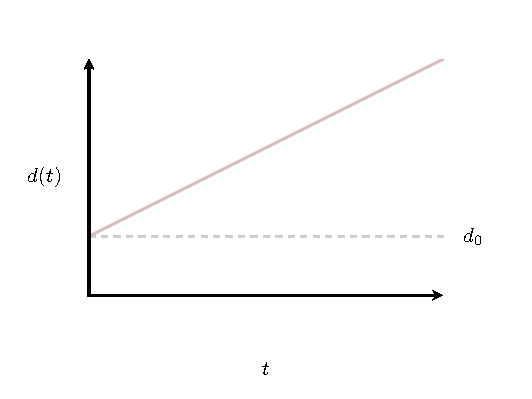
\includegraphics[width=0.75\textwidth,height=\textheight]{figures/growth/linear/linear.pdf}

}

\caption{\label{fig-linear}In a linear growth model a tree diameter
grows linear with time.}

\end{figure}

Linear diameter growth over an extended time is often unrealistic, but
it can be a reasonable approximation for more complicated growth
dynamics over shorter intervals of time.

\hypertarget{linear-mass-growth}{%
\subsubsection{Linear Mass Growth}\label{linear-mass-growth}}

Linear diameter growth, however, also has awkward physiological
consequences. As a tree grows a fixed increase in diameter requires
larger and larger increases in overall mass.

If the energy inputs to a tree are fixed then an arguably more realistic
model would assume that mass, and not diameter, increases linearly with
time. To model this mathematically let's assume that we can approximate
trees as cylinders with constant density so that the total mass is
related to the diameter by \begin{align*}
m
&=
\text{density} \cdot \text{volume}
\\
&=
\rho \cdot \pi \, \left( \frac{d}{2} \right)^{2} \, h
\\
&=
\left( \frac{\pi}{4} \cdot \rho \cdot h \right) \, d^{2}
\\
&=
C \, d^{2}.
\end{align*} For convenience I've absorbed everything but the diameter
into a single constant in that last step.

If the tree mass grows linearly with time and the height remaining
constant then \begin{align*}
\delta m \cdot t
&=
m(t) - m_{0}
\\
&=
C \, d(t)^{2} - C \, d_{0}^{2},
\end{align*} or upon solving for \(d(t)\), \begin{align*}
\delta m \cdot t
&=
C \, d(t)^{2} - C \, d_{0}^{2}
\\
\frac{\delta m}{C} \cdot t
&=
d(t)^{2} - d_{0}^{2}
\\
d(t)^{2}
&=
d_{0}^{2} + \frac{\delta m}{C} \cdot t
\\
d(t)
&=
\sqrt{ d_{0}^{2} + \frac{\delta m}{C} \cdot t }
\\
d(t)
&=
\sqrt{ d_{0}^{2} + \beta \cdot t }.
\end{align*} Because of the square root function the diameter growth
will decelerate as a tree ages, but never quite stop
(Figure~\ref{fig-square-root}).

\begin{figure}

{\centering 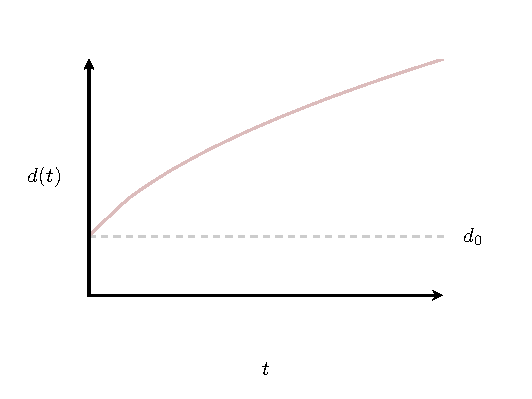
\includegraphics[width=0.75\textwidth,height=\textheight]{figures/growth/square_root/square_root.pdf}

}

\caption{\label{fig-square-root}Under idealized assumptions a linear
increase in the mass of a tree results in a square root increase in the
diameter of the tree.}

\end{figure}

\hypertarget{gompertz-model}{%
\subsubsection{Gompertz Model}\label{gompertz-model}}

In practice both the linear and square root growth models will be too
inflexible to adequately model tree diameter growth for the decades that
our observations span. One particularly common class of models assume
that the diameter growth follows a \emph{sigmoidal curve}, allowing for
accelerated growth at early ages, constant growth at intermediate ages,
and decelerating growth at later ages. There are many mathematical
curves that fit this qualitative shape, but a particularly common choice
in many ecological applications is the \textbf{Gompertz} family of
curves, \[
d(t) = d_{\max} \, \exp( -b \exp( -c \, t) ).
\] To ensure monotonically increasing growth all three parameters must
be positive.

The interpretation of the parameter \(d_{\max}\) is straightforward: it
determines the asymptotic diameter that a tree will approach as it ages.
On the other hand the interpretation of the other two parameters is less
clear, which can frustrate a principled use of this model in a real
analysis.

One way to make the Gompertz family of curves more interpretable is to
find an alternative parameterization where each parameter directly
corresponds to a meaningful behavior. For example we might parameterize
the curves in terms of their linear behavior at intermediate times.

To that end let's introduce the intermediate time \(\tau\) where a given
Gompertz curve reached half of its asymptotic diameter, \[
\frac{ d_{\max} }{ 2 }
= d(\tau)
= d_{\max} \exp( -b \exp( -c \, \tau) ),
\] or, solving for \(\tau\), \[
\tau = \frac{ \log b - \log \log 2 }{ c }.
\] The rate of growth at \(\tau\) is then given by \[
\beta
= \frac{ \mathrm{d} d }{ \mathrm{d} t }(\tau)
= \frac{ \log 2 }{ 2 } d_{\max} \, c.
\]

Conveniently the tree values \(d_{\max}\), \(\tau\), and \(\beta\)
completely determine a Gompertz curve. In terms of these parameters the
Gompertz family of curves becomes (Figure~\ref{fig-gompertz}) \[
d(t) = d_{\max} \,
\exp \left( -\log 2 \cdot
\exp \left( -\frac{2}{\log 2} \, \frac{\beta}{d_{\max}} \,
             \left( t - \tau \right) \right)
\right)
\] which is fortunately straightforward to implement in practice.

\begin{figure}

{\centering 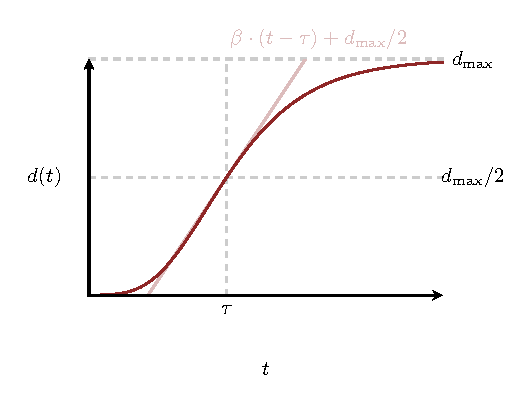
\includegraphics[width=0.75\textwidth,height=\textheight]{figures/growth/gompertz/gompertz.pdf}

}

\caption{\label{fig-gompertz}The Gompertz family of curves provides a
sigmoidal model for tree diameter growth. Here we've parameterized each
curve in terms of its asymptotic diameter, \(d_{\max}\), the time at
which curve reaches half of this value, \(\tau\), and the derivative at
\(\tau\), \(\beta\).}

\end{figure}

There are many ways of adding more flexible to the Gompertz model that
could be useful when analyzing tree growth data. For example replacing
\(t - \tau\) with a polynomial would allow for more complicated,
potentially even asymmetric, behavior at both young and old ages. Here
we will consider a less sophisticated addition: a non-zero initial
diameter, \[
d(t) = d_{0} + \delta d \,
\exp \left( -\log 2 \cdot
\exp \left( -\frac{2}{\log 2} \, \frac{\beta}{\delta d} \,
             \left( t - \tau \right) \right).
\right)
\] This offset could, for instance, allow the model to accommodate
different growth dynamics for very young trees before sigmoidal growth
kicks in.

\hypertarget{measurement-model}{%
\subsection{Measurement Model}\label{measurement-model}}

Now that we have some candidate models for how tree diameter grows with
time we need to consider how those diameters are actually measured.

The diameter at breast height measurement procedure is not infinitely
precise. There can be errors in reading the measuring tape,
misalignments of the measuring tape, non-uniforming in the diameter of
the tree, inconsistencies from measurement to measurement, and more. A
useful measurement model needs to account for not only how strongly
these potential sources of variation can affect the diameter at breast
height measurements but also what overall variation is consistent with
our understanding of the procedure.

For example let's consider how much misalignment of the measuring tape
can affect diameter measurements. As we did in the linear mass growth
model let's assume that trees are well approximated by a cylinder of
radius \(r\), diameter \(d = 2 \, r\), and height \(h\), with all
lengths in units of centimeters.

In a perfect diameter at breast height measurement the measuring tape
will form a circle with the same circumference as the tree at the tag
height. Consequently we can recover the diameter of the tree by dividing
the measured length by \(\pi\), \[
d = \frac{ C_{\mathrm{flat}} }{ \pi }.
\]

When tape is tilted, however, it will form not a circle but rather an
\emph{ellipse}. If the maximum offset is given by \(\delta\) then the
shape of the ellipse will be determined by the semi-minor axis
(Figure~\ref{fig-measurement}) \[
b = r = \frac{d}{2}
\] and the semi-major axis \[
a = \frac{1}{2} \sqrt{ d^{2} + \delta^{2} }.
\] As we would hope this reduces back to a circle with \(a = b = r\)
when \(\delta \rightarrow 0\).

\begin{figure}

{\centering 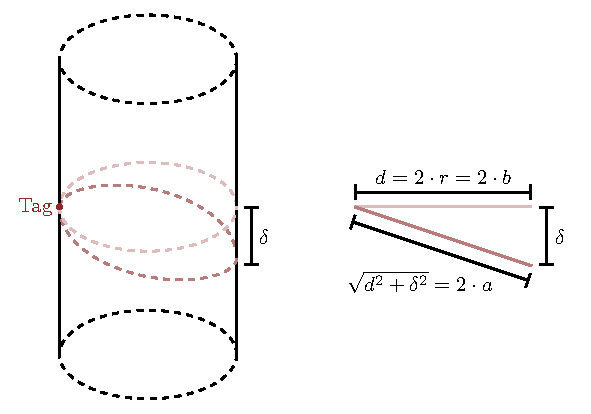
\includegraphics[width=0.75\textwidth,height=\textheight]{figures/diameter_measurement_error/diameter_measurement_error.pdf}

}

\caption{\label{fig-measurement}When misaligned a measuring tape wrapped
around a cylindrical tree defines an ellipse. In this case dividing the
measured length by \(\pi\) does not give the tree diameter exactly.}

\end{figure}

Unfortunately the perimeter of an ellipse does not admit a simple
mathematical form; instead it is given by a complicated function known
as an \textbf{elliptic integral}. For those interested in learning more
Wikipedia has a nice discussion at
\url{https://en.wikipedia.org/wiki/Ellipse\#Circumference}. We can,
however, \emph{approximate} the perimeter of an ellipse is a variety of
different ways; again Wikipedia has a clear discussion,
\url{https://en.wikipedia.org/wiki/Ellipse\#Arc_length}.

For example the circumference of this tilted ellipse can be bounded
above by \begin{align*}
C_{\mathrm{tilt}}
&\le
\sqrt{2} \, \pi \, \sqrt{ b^{2} + a^{2} }
\\
&\le
\sqrt{2} \, \pi \,
\sqrt{  \left( \frac{d}{2} \right)^{2}
      + \left(\frac{1}{2}\right)^{2} \bigg( d^{2} + \delta^{2} \bigg)
}
\\
&\le
\sqrt{2} \, \pi \, \frac{1}{2} \sqrt{ d^{2} + d^{2} + \delta^{2} }
\\
&\le
\sqrt{2} \, \pi \, \frac{1}{2} \sqrt{ 2 d^{2} + \delta^{2} }
\\
&\le
\sqrt{2} \, \pi \, \frac{\sqrt{2} \, d}{2}
\sqrt{ 1 + \left( \frac{\delta}{2 \, d} \right)^{2} }
\\
&\le
\pi \, d \, \sqrt{ 1 + \left( \frac{\delta}{2 \, d} \right)^{2} }.
\end{align*} If the offset \(\delta\) is much smaller than the actual
tree diameter \(d\) then this upper bound will be a useful conservative
approximation to the exact length of the tilted measuring tape, \[
C_{\mathrm{tilt}} \approx
\pi \, d \, \sqrt{ 1 + \left( \frac{\delta}{2 \, d} \right)^{2} }.
\]

Using the perimeter of the tilted ellipse in place of the perimeter of a
flat circle does not recover the diameter of the tree, \[
\frac{C_{\mathrm{tilt}}}{\pi}
=
d \, \sqrt{ 1 + \left( \frac{\delta}{2 \, d} \right)^{2} } \ge d.
\] The larger perimeter always biases the recovered diameter to larger
values. When \(\delta\) is unknown this bias manifests as an asymmetric
variability in the measurements.

Note that this measurement variability is not additive but rather
\emph{multiplicative}. Indeed multiplicative measurement variability is
common when working with measurements of positive quantities. One way to
recover additive measurement variability is to work with log diameters,
\[
\log \frac{C_{\mathrm{tilt}}}{\pi}
=
\log d
+ \frac{1}{2}
  \log \left( 1 + \left( \frac{\delta}{2 \, d} \right)^{2} \right).
\]

In practice we can sometimes approximate the multiplicative measurement
variability with additive measurement variability, \[
\frac{C_{\mathrm{tilt}}}{\pi} \approx
d
+ d_{0}
  \left( \sqrt{ 1 + \left( \frac{\delta}{2 \, d} \right)^{2} } - 1 \right),
\] where \(d_{0}\) is the baseline diameter at which we want this
approximation to be best. This approximation is decent if all of our
measurements are limited to a narrow range of tree diameters, but if our
data spans measurements of very small and very large trees then the
approximation can break down at the extremes.

Assuming that an additive measurement model is a good enough
approximation what do these variabilities look like in practice? If the
offsets never exceed ten percent of the actual tree diameter, which
allows for some pretty strong misalignments, then \[
\frac{ \delta }{ d } \approx 0.1,
\] \[
\frac{ \delta }{ 2 \, d } \approx 0.05,
\] and \[
\sqrt{ 1 + \left( \frac{\delta}{2 \, d} \right)^{2} } \approx 1.001.
\] The deviation from the measured diameter to the true diameter is
exceedingly small!

For example if \(d_{0} = 50 \, \mathrm{cm}\) then the scale of the
approximate additive measurement variability would be orders of
magnitude smaller, \[
d_{0}
\left( \sqrt{ 1 + \left( \frac{\delta}{2 \, d} \right)^{2} } - 1 \right)
\approx 0.05 \, \mathrm{cm},
\] which we can round up to about a millimeter. This may appear
surprisingly small but it's all a consequence of the geometry:
relatively large warpings of a circle don't change the diameter as much
as we might expect!

Analysis of the other potential sources of variation gives similar
results: multiplicative variation is more realistic but additive
variation can be a reasonable approximation, and the scale of the linear
variation is unlikely to exceed a millimeter or so. For this exercise
we'll assume the simpler linear measurement model, \[
\hat{d}(t) \sim \text{normal}(d(t), \sigma),
\] with our domain expertise excluding values of \(\sigma\) much larger
than \(0.1 \, \mathrm{cm}\). To be particularly conservative we will
allow for measurement variabilities as large as \(0.25 \, \mathrm{cm}\).

\hypertarget{sec:analyses}{%
\section{Demonstrative Analyses}\label{sec:analyses}}

Having brainstormed some possible models let's try to incorporate them
into a Bayesian analysis using the probabilistic programming tool
\texttt{Stan}, in particular it's \texttt{R} interface \texttt{RStan}.

\hypertarget{sec:setup}{%
\subsection{Set Up}\label{sec:setup}}

First and foremost we need to load the \texttt{rstan} package into our
local \texttt{R} environment and configure it.

\begin{Shaded}
\begin{Highlighting}[]
\FunctionTok{library}\NormalTok{(rstan)}
\FunctionTok{rstan\_options}\NormalTok{(}\AttributeTok{auto\_write =} \ConstantTok{TRUE}\NormalTok{)            }\CommentTok{\# Cache compiled Stan programs}
\FunctionTok{options}\NormalTok{(}\AttributeTok{mc.cores =}\NormalTok{ parallel}\SpecialCharTok{::}\FunctionTok{detectCores}\NormalTok{()) }\CommentTok{\# Parallelize chains}
\NormalTok{parallel}\SpecialCharTok{:::}\FunctionTok{setDefaultClusterOptions}\NormalTok{(}\AttributeTok{setup\_strategy =} \StringTok{"sequential"}\NormalTok{)}
\end{Highlighting}
\end{Shaded}

Next we'll load my recommended Markov chain Monte Carlo diagnostic and
analysis code. The code itself as well as documentation can be found at
\url{https://github.com/betanalpha/mcmc_diagnostics}.

\begin{Shaded}
\begin{Highlighting}[]
\NormalTok{util }\OtherTok{\textless{}{-}} \FunctionTok{new.env}\NormalTok{()}
\FunctionTok{source}\NormalTok{(}\StringTok{\textquotesingle{}stan\_utility\_rstan.R\textquotesingle{}}\NormalTok{, }\AttributeTok{local=}\NormalTok{util)}
\end{Highlighting}
\end{Shaded}

\hypertarget{sec:homo-linear}{%
\subsection{Homogeneous Linear Model}\label{sec:homo-linear}}

Let's start as simply as possible: we'll assume a linear diameter growth
model where all trees in the data set are allowed to have different
initial diameters but all grow at the same rate. I will use normal
containment prior models to softly constrain the initial heights below
150 cm, the growth rate below 2 cm per year in magnitude, and the
measurement variability below 0.25 cm. For an introduction to normal
containment prior models see
\url{https://betanalpha.github.io/assets/case_studies/prior_modeling.html\#3_One-Dimensional_Expertise}.

To facilitate the analysis of our Stan program we will also save the
inferred diameter of each tree along a grid of times.

\begin{codelisting}

\caption{\texttt{homogeneous\_linear\_growth.stan}}

\begin{Shaded}
\begin{Highlighting}[]
\KeywordTok{data}\NormalTok{ \{}
  \DataTypeTok{int}\NormalTok{\textless{}}\KeywordTok{lower}\NormalTok{=}\DecValTok{1}\NormalTok{\textgreater{} N;}
  \DataTypeTok{int}\NormalTok{\textless{}}\KeywordTok{lower}\NormalTok{=}\DecValTok{1}\NormalTok{\textgreater{} N\_trees;}
  \DataTypeTok{int}\NormalTok{\textless{}}\KeywordTok{lower}\NormalTok{=}\DecValTok{1}\NormalTok{\textgreater{} tree\_N\_obs[N\_trees];}
  \DataTypeTok{int}\NormalTok{\textless{}}\KeywordTok{lower}\NormalTok{=}\DecValTok{1}\NormalTok{, }\KeywordTok{upper}\NormalTok{=N\textgreater{} tree\_start\_idxs[N\_trees];}
  \DataTypeTok{int}\NormalTok{\textless{}}\KeywordTok{lower}\NormalTok{=}\DecValTok{1}\NormalTok{, }\KeywordTok{upper}\NormalTok{=N\textgreater{} tree\_end\_idxs[N\_trees];}
  \DataTypeTok{vector}\NormalTok{[N] tree\_years;}
  \DataTypeTok{vector}\NormalTok{[N] tree\_dbhs;}
  
  \DataTypeTok{int}\NormalTok{\textless{}}\KeywordTok{lower}\NormalTok{=}\DecValTok{1}\NormalTok{\textgreater{} N\_year\_grid;}
  \DataTypeTok{vector}\NormalTok{[N\_year\_grid] year\_grid;}
\NormalTok{\}}

\KeywordTok{parameters}\NormalTok{ \{}
  \DataTypeTok{real}\NormalTok{\textless{}}\KeywordTok{lower}\NormalTok{=}\DecValTok{0}\NormalTok{\textgreater{} d0[N\_trees]; }\CommentTok{// Diameter at year of first observation (cm)}
  \DataTypeTok{real}\NormalTok{ beta;                 }\CommentTok{// Linear growth rate (cm / year)}
  \DataTypeTok{real}\NormalTok{\textless{}}\KeywordTok{lower}\NormalTok{=}\DecValTok{0}\NormalTok{\textgreater{} sigma;       }\CommentTok{// Measurement variability (cm)}
\NormalTok{\}}

\KeywordTok{model}\NormalTok{ \{}
\NormalTok{  d0 \textasciitilde{} normal(}\DecValTok{0}\NormalTok{, }\DecValTok{150}\NormalTok{ / }\FloatTok{2.57}\NormalTok{);     }\CommentTok{// 99\% prior mass between 0 and 150 cm}
\NormalTok{  beta \textasciitilde{} normal(}\DecValTok{0}\NormalTok{, }\DecValTok{2}\NormalTok{ / }\FloatTok{2.32}\NormalTok{);     }\CommentTok{// 99\% prior mass between +/{-} 2 cm / year}
\NormalTok{  sigma \textasciitilde{} normal(}\DecValTok{0}\NormalTok{, }\FloatTok{0.25}\NormalTok{ / }\FloatTok{2.57}\NormalTok{); }\CommentTok{// 99\% prior mass between 0 and 0.25 cm }
  
  \ControlFlowTok{for}\NormalTok{ (t }\ControlFlowTok{in} \DecValTok{1}\NormalTok{:N\_trees) \{}
    \DataTypeTok{int}\NormalTok{ start\_idx = tree\_start\_idxs[t];}
    \DataTypeTok{int}\NormalTok{ end\_idx = tree\_end\_idxs[t];}
    \DataTypeTok{vector}\NormalTok{[tree\_N\_obs[t]] years = tree\_years[start\_idx:end\_idx];}
    \DataTypeTok{vector}\NormalTok{[tree\_N\_obs[t]] dbhs = tree\_dbhs[start\_idx:end\_idx];}
    
\NormalTok{    dbhs \textasciitilde{} normal(d0[t] + beta * (years {-} years[}\DecValTok{1}\NormalTok{]), sigma);}
\NormalTok{  \}}
\NormalTok{\}}

\KeywordTok{generated quantities}\NormalTok{ \{}
  \DataTypeTok{real}\NormalTok{ dbh\_grid\_pred[N\_trees, N\_year\_grid];}
  \ControlFlowTok{for}\NormalTok{ (t }\ControlFlowTok{in} \DecValTok{1}\NormalTok{:N\_trees) \{}
    \DataTypeTok{real}\NormalTok{ y0 = tree\_years[tree\_start\_idxs[t]];}
    \ControlFlowTok{for}\NormalTok{ (n }\ControlFlowTok{in} \DecValTok{1}\NormalTok{:N\_year\_grid) \{}
      \DataTypeTok{real}\NormalTok{ mu = d0[t] + beta * (year\_grid[n] {-} y0);}
\NormalTok{      dbh\_grid\_pred[t, n] = normal\_rng(mu, sigma);}
\NormalTok{    \}}
\NormalTok{  \}}
\NormalTok{\}}
\end{Highlighting}
\end{Shaded}

\end{codelisting}

\begin{Shaded}
\begin{Highlighting}[]
\NormalTok{data }\OtherTok{\textless{}{-}} \FunctionTok{mget}\NormalTok{(}\FunctionTok{c}\NormalTok{(}\StringTok{"N"}\NormalTok{, }\StringTok{"N\_trees"}\NormalTok{, }\StringTok{"tree\_N\_obs"}\NormalTok{,}
               \StringTok{"tree\_start\_idxs"}\NormalTok{, }\StringTok{"tree\_end\_idxs"}\NormalTok{,}
               \StringTok{"tree\_years"}\NormalTok{, }\StringTok{"tree\_dbhs"}\NormalTok{))}

\NormalTok{year\_grid }\OtherTok{\textless{}{-}} \FunctionTok{seq}\NormalTok{(}\DecValTok{1975}\NormalTok{, }\DecValTok{2020}\NormalTok{, }\DecValTok{1}\NormalTok{)}
\NormalTok{N\_year\_grid }\OtherTok{\textless{}{-}} \FunctionTok{length}\NormalTok{(year\_grid)}

\NormalTok{data}\SpecialCharTok{$}\NormalTok{N\_year\_grid }\OtherTok{\textless{}{-}}\NormalTok{ N\_year\_grid}
\NormalTok{data}\SpecialCharTok{$}\NormalTok{year\_grid }\OtherTok{\textless{}{-}}\NormalTok{ year\_grid}
\end{Highlighting}
\end{Shaded}

\begin{Shaded}
\begin{Highlighting}[]
\NormalTok{fit }\OtherTok{\textless{}{-}} \FunctionTok{stan}\NormalTok{(}\AttributeTok{file=}\StringTok{"stan\_programs/homogeneous\_linear\_growth.stan"}\NormalTok{,}
            \AttributeTok{data=}\NormalTok{data, }\AttributeTok{seed=}\DecValTok{8438338}\NormalTok{,}
            \AttributeTok{warmup=}\DecValTok{1000}\NormalTok{, }\AttributeTok{iter=}\DecValTok{2024}\NormalTok{, }\AttributeTok{refresh=}\DecValTok{0}\NormalTok{)}
\end{Highlighting}
\end{Shaded}

The lack of diagnostic failures is consistent with \texttt{Stan} being
able to accurately quantify our posterior uncertainties.

\begin{Shaded}
\begin{Highlighting}[]
\NormalTok{diagnostics }\OtherTok{\textless{}{-}}\NormalTok{ util}\SpecialCharTok{$}\FunctionTok{extract\_hmc\_diagnostics}\NormalTok{(fit)}
\NormalTok{util}\SpecialCharTok{$}\FunctionTok{check\_all\_hmc\_diagnostics}\NormalTok{(diagnostics)}
\end{Highlighting}
\end{Shaded}

\begin{verbatim}
  All Hamiltonian Monte Carlo diagnostics are consistent with reliable
Markov chain Monte Carlo.
\end{verbatim}

\begin{Shaded}
\begin{Highlighting}[]
\NormalTok{samples }\OtherTok{\textless{}{-}}\NormalTok{ util}\SpecialCharTok{$}\FunctionTok{extract\_expectands}\NormalTok{(fit)}
\NormalTok{base\_samples }\OtherTok{\textless{}{-}}\NormalTok{ util}\SpecialCharTok{$}\FunctionTok{filter\_expectands}\NormalTok{(samples,}
                                       \FunctionTok{c}\NormalTok{(}\StringTok{\textquotesingle{}d0\textquotesingle{}}\NormalTok{, }\StringTok{\textquotesingle{}beta\textquotesingle{}}\NormalTok{, }\StringTok{\textquotesingle{}sigma\textquotesingle{}}\NormalTok{),}
                                       \AttributeTok{check\_arrays=}\ConstantTok{TRUE}\NormalTok{)}
\NormalTok{util}\SpecialCharTok{$}\FunctionTok{check\_all\_expectand\_diagnostics}\NormalTok{(base\_samples)}
\end{Highlighting}
\end{Shaded}

\begin{verbatim}
All expectands checked appear to be behaving well enough for reliable
Markov chain Monte Carlo estimation.
\end{verbatim}

Unfortunately posterior retrodictive checks show a poor fit for many of
the trees in our data set. This suggests that different trees might be
growing at different rates.

\begin{Shaded}
\begin{Highlighting}[]
\NormalTok{plot\_cont\_marginal\_quantiles }\OtherTok{\textless{}{-}} \ControlFlowTok{function}\NormalTok{(xs, preds,}
                                         \AttributeTok{display\_xlims=}\ConstantTok{NA}\NormalTok{,}
                                         \AttributeTok{display\_ylims=}\ConstantTok{NA}\NormalTok{,}
                                         \AttributeTok{title=}\StringTok{""}\NormalTok{,}
                                         \AttributeTok{x\_name=}\StringTok{""}\NormalTok{, }\AttributeTok{y\_name=}\StringTok{""}\NormalTok{) \{}
\NormalTok{  probs }\OtherTok{=} \FunctionTok{c}\NormalTok{(}\FloatTok{0.1}\NormalTok{, }\FloatTok{0.2}\NormalTok{, }\FloatTok{0.3}\NormalTok{, }\FloatTok{0.4}\NormalTok{, }\FloatTok{0.5}\NormalTok{, }\FloatTok{0.6}\NormalTok{, }\FloatTok{0.7}\NormalTok{, }\FloatTok{0.8}\NormalTok{, }\FloatTok{0.9}\NormalTok{)}
\NormalTok{  cred }\OtherTok{\textless{}{-}} \FunctionTok{sapply}\NormalTok{(preds, }\ControlFlowTok{function}\NormalTok{(pred)}
                        \FunctionTok{quantile}\NormalTok{(}\FunctionTok{c}\NormalTok{(}\FunctionTok{t}\NormalTok{(pred), }\AttributeTok{recursive=}\ConstantTok{TRUE}\NormalTok{),}
                        \AttributeTok{probs=}\NormalTok{probs))}

  \ControlFlowTok{if}\NormalTok{ (}\FunctionTok{is.na}\NormalTok{(display\_xlims)) \{}
\NormalTok{    xlims }\OtherTok{\textless{}{-}} \FunctionTok{range}\NormalTok{(xs)}
\NormalTok{  \} }\ControlFlowTok{else}\NormalTok{ \{}
\NormalTok{    xlims }\OtherTok{\textless{}{-}}\NormalTok{ display\_xlims}
\NormalTok{  \}}

  \ControlFlowTok{if}\NormalTok{ (}\FunctionTok{is.na}\NormalTok{(display\_ylims)) \{}
\NormalTok{    ylims }\OtherTok{\textless{}{-}} \FunctionTok{c}\NormalTok{(}\FunctionTok{min}\NormalTok{(cred[}\DecValTok{1}\NormalTok{,]), }\FunctionTok{max}\NormalTok{(cred[}\DecValTok{9}\NormalTok{,]))}
\NormalTok{  \} }\ControlFlowTok{else}\NormalTok{ \{}
\NormalTok{    ylims }\OtherTok{\textless{}{-}}\NormalTok{ display\_ylims}
\NormalTok{  \}}

  \FunctionTok{plot}\NormalTok{(}\DecValTok{1}\NormalTok{, }\AttributeTok{type=}\StringTok{"n"}\NormalTok{, }\AttributeTok{main=}\NormalTok{title,}
       \AttributeTok{xlim=}\NormalTok{xlims, }\AttributeTok{xlab=}\NormalTok{x\_name,}
       \AttributeTok{ylim=}\NormalTok{ylims, }\AttributeTok{ylab=}\NormalTok{y\_name)}

  \FunctionTok{polygon}\NormalTok{(}\FunctionTok{c}\NormalTok{(xs, }\FunctionTok{rev}\NormalTok{(xs)), }\FunctionTok{c}\NormalTok{(cred[}\DecValTok{1}\NormalTok{,], }\FunctionTok{rev}\NormalTok{(cred[}\DecValTok{9}\NormalTok{,])),}
          \AttributeTok{col =}\NormalTok{ c\_light, }\AttributeTok{border =} \ConstantTok{NA}\NormalTok{)}
  \FunctionTok{polygon}\NormalTok{(}\FunctionTok{c}\NormalTok{(xs, }\FunctionTok{rev}\NormalTok{(xs)), }\FunctionTok{c}\NormalTok{(cred[}\DecValTok{2}\NormalTok{,], }\FunctionTok{rev}\NormalTok{(cred[}\DecValTok{8}\NormalTok{,])),}
          \AttributeTok{col =}\NormalTok{ c\_light\_highlight, }\AttributeTok{border =} \ConstantTok{NA}\NormalTok{)}
  \FunctionTok{polygon}\NormalTok{(}\FunctionTok{c}\NormalTok{(xs, }\FunctionTok{rev}\NormalTok{(xs)), }\FunctionTok{c}\NormalTok{(cred[}\DecValTok{3}\NormalTok{,], }\FunctionTok{rev}\NormalTok{(cred[}\DecValTok{7}\NormalTok{,])),}
          \AttributeTok{col =}\NormalTok{ c\_mid, }\AttributeTok{border =} \ConstantTok{NA}\NormalTok{)}
  \FunctionTok{polygon}\NormalTok{(}\FunctionTok{c}\NormalTok{(xs, }\FunctionTok{rev}\NormalTok{(xs)), }\FunctionTok{c}\NormalTok{(cred[}\DecValTok{4}\NormalTok{,], }\FunctionTok{rev}\NormalTok{(cred[}\DecValTok{6}\NormalTok{,])),}
          \AttributeTok{col =}\NormalTok{ c\_mid\_highlight, }\AttributeTok{border =} \ConstantTok{NA}\NormalTok{)}
  \FunctionTok{lines}\NormalTok{(xs, cred[}\DecValTok{5}\NormalTok{,], }\AttributeTok{col=}\NormalTok{c\_dark, }\AttributeTok{lwd=}\DecValTok{2}\NormalTok{)}
\NormalTok{\}}

\FunctionTok{par}\NormalTok{(}\AttributeTok{mfrow=}\FunctionTok{c}\NormalTok{(}\DecValTok{3}\NormalTok{, }\DecValTok{3}\NormalTok{), }\AttributeTok{mar =} \FunctionTok{c}\NormalTok{(}\DecValTok{5}\NormalTok{, }\DecValTok{4}\NormalTok{, }\DecValTok{2}\NormalTok{, }\DecValTok{1}\NormalTok{))}

\ControlFlowTok{for}\NormalTok{ (t }\ControlFlowTok{in} \DecValTok{1}\SpecialCharTok{:}\NormalTok{data}\SpecialCharTok{$}\NormalTok{N\_trees) \{}
\NormalTok{  idxs }\OtherTok{\textless{}{-}}\NormalTok{ data}\SpecialCharTok{$}\NormalTok{tree\_start\_idxs[t]}\SpecialCharTok{:}\NormalTok{data}\SpecialCharTok{$}\NormalTok{tree\_end\_idxs[t]}
\NormalTok{  years }\OtherTok{\textless{}{-}}\NormalTok{ data}\SpecialCharTok{$}\NormalTok{tree\_years[idxs]}
\NormalTok{  dbhs }\OtherTok{\textless{}{-}}\NormalTok{ data}\SpecialCharTok{$}\NormalTok{tree\_dbhs[idxs]}

\NormalTok{  pred\_names }\OtherTok{\textless{}{-}} \FunctionTok{sapply}\NormalTok{(}\DecValTok{1}\SpecialCharTok{:}\NormalTok{data}\SpecialCharTok{$}\NormalTok{N\_year\_grid,}
                       \ControlFlowTok{function}\NormalTok{(n) }\FunctionTok{paste0}\NormalTok{(}\StringTok{\textquotesingle{}dbh\_grid\_pred[\textquotesingle{}}\NormalTok{,}
\NormalTok{                                          t, }\StringTok{\textquotesingle{},\textquotesingle{}}\NormalTok{, n, }\StringTok{\textquotesingle{}]\textquotesingle{}}\NormalTok{))}
\NormalTok{  preds }\OtherTok{\textless{}{-}}\NormalTok{ samples[pred\_names]}
  \FunctionTok{plot\_cont\_marginal\_quantiles}\NormalTok{(data}\SpecialCharTok{$}\NormalTok{year\_grid, preds,}
                               \AttributeTok{title=}\FunctionTok{paste0}\NormalTok{(tree\_ids[t], }\StringTok{", t = "}\NormalTok{, t),}
                               \AttributeTok{x\_name=}\StringTok{"Year"}\NormalTok{, }\AttributeTok{y\_name=}\StringTok{"DBH (cm)"}\NormalTok{)}
  \FunctionTok{points}\NormalTok{(years, dbhs, }\AttributeTok{col=}\StringTok{"white"}\NormalTok{, }\AttributeTok{pch=}\DecValTok{16}\NormalTok{, }\AttributeTok{cex=}\FloatTok{1.2}\NormalTok{)}
  \FunctionTok{points}\NormalTok{(years, dbhs, }\AttributeTok{col=}\StringTok{"black"}\NormalTok{, }\AttributeTok{pch=}\DecValTok{16}\NormalTok{, }\AttributeTok{cex=}\FloatTok{0.8}\NormalTok{)}
\NormalTok{\}}
\end{Highlighting}
\end{Shaded}

\begin{figure}[H]

{\centering \includegraphics{tree_diameter_growth_analysis_files/figure-pdf/unnamed-chunk-19-1.pdf}

}

\end{figure}

\begin{figure}[H]

{\centering \includegraphics{tree_diameter_growth_analysis_files/figure-pdf/unnamed-chunk-19-2.pdf}

}

\end{figure}

The inadequacy of this first model is also hinted at in the inferred
posterior behavior. Marginal posterior distributions for all of the
initial diameters appears to be reasonable.

\begin{Shaded}
\begin{Highlighting}[]
\NormalTok{plot\_disc\_marginal\_quantiles }\OtherTok{\textless{}{-}} \ControlFlowTok{function}\NormalTok{(samples, names, }\AttributeTok{x\_name=}\StringTok{""}\NormalTok{) \{}
\NormalTok{  N }\OtherTok{\textless{}{-}} \FunctionTok{length}\NormalTok{(names)}
\NormalTok{  idx }\OtherTok{\textless{}{-}} \FunctionTok{rep}\NormalTok{(}\DecValTok{1}\SpecialCharTok{:}\NormalTok{N, }\AttributeTok{each=}\DecValTok{2}\NormalTok{)}
\NormalTok{  xs }\OtherTok{\textless{}{-}} \FunctionTok{sapply}\NormalTok{(}\DecValTok{1}\SpecialCharTok{:}\FunctionTok{length}\NormalTok{(idx), }\ControlFlowTok{function}\NormalTok{(k)}
                              \ControlFlowTok{if}\NormalTok{(k }\SpecialCharTok{\%\%} \DecValTok{2} \SpecialCharTok{==} \DecValTok{0}\NormalTok{) idx[k] }\SpecialCharTok{+} \FloatTok{0.5} \ControlFlowTok{else}\NormalTok{ idx[k] }\SpecialCharTok{{-}} \FloatTok{0.5}\NormalTok{)}

\NormalTok{  probs }\OtherTok{=} \FunctionTok{c}\NormalTok{(}\FloatTok{0.1}\NormalTok{, }\FloatTok{0.2}\NormalTok{, }\FloatTok{0.3}\NormalTok{, }\FloatTok{0.4}\NormalTok{, }\FloatTok{0.5}\NormalTok{, }\FloatTok{0.6}\NormalTok{, }\FloatTok{0.7}\NormalTok{, }\FloatTok{0.8}\NormalTok{, }\FloatTok{0.9}\NormalTok{)}
\NormalTok{  cred }\OtherTok{\textless{}{-}} \FunctionTok{sapply}\NormalTok{(}\DecValTok{1}\SpecialCharTok{:}\NormalTok{N, }\ControlFlowTok{function}\NormalTok{(n)}
                      \FunctionTok{quantile}\NormalTok{(}\FunctionTok{c}\NormalTok{(}\FunctionTok{t}\NormalTok{(samples[[names[n]]]), }\AttributeTok{recursive=}\ConstantTok{TRUE}\NormalTok{),}
                               \AttributeTok{probs=}\NormalTok{probs))}
\NormalTok{  pad\_cred }\OtherTok{\textless{}{-}} \FunctionTok{do.call}\NormalTok{(cbind, }\FunctionTok{lapply}\NormalTok{(idx, }\ControlFlowTok{function}\NormalTok{(n) cred[}\DecValTok{1}\SpecialCharTok{:}\DecValTok{9}\NormalTok{,n]))}

\NormalTok{  ylims }\OtherTok{\textless{}{-}} \FunctionTok{c}\NormalTok{(}\FunctionTok{min}\NormalTok{(cred[}\DecValTok{1}\NormalTok{,]), }\FunctionTok{max}\NormalTok{(cred[}\DecValTok{9}\NormalTok{,]))}

  \FunctionTok{plot}\NormalTok{(}\DecValTok{1}\NormalTok{, }\AttributeTok{type=}\StringTok{"n"}\NormalTok{,}
       \AttributeTok{xlim=}\FunctionTok{c}\NormalTok{(}\FloatTok{0.5}\NormalTok{, N }\SpecialCharTok{+} \FloatTok{0.5}\NormalTok{), }\AttributeTok{xlab=}\NormalTok{x\_name,}
       \AttributeTok{ylim=}\NormalTok{ylims, }\AttributeTok{ylab=}\StringTok{"Marginal}\SpecialCharTok{\textbackslash{}n}\StringTok{Posterior Quantiles"}\NormalTok{)}

  \FunctionTok{polygon}\NormalTok{(}\FunctionTok{c}\NormalTok{(xs, }\FunctionTok{rev}\NormalTok{(xs)), }\FunctionTok{c}\NormalTok{(pad\_cred[}\DecValTok{1}\NormalTok{,], }\FunctionTok{rev}\NormalTok{(pad\_cred[}\DecValTok{9}\NormalTok{,])),}
          \AttributeTok{col =}\NormalTok{ c\_light, }\AttributeTok{border =} \ConstantTok{NA}\NormalTok{)}
  \FunctionTok{polygon}\NormalTok{(}\FunctionTok{c}\NormalTok{(xs, }\FunctionTok{rev}\NormalTok{(xs)), }\FunctionTok{c}\NormalTok{(pad\_cred[}\DecValTok{2}\NormalTok{,], }\FunctionTok{rev}\NormalTok{(pad\_cred[}\DecValTok{8}\NormalTok{,])),}
          \AttributeTok{col =}\NormalTok{ c\_light\_highlight, }\AttributeTok{border =} \ConstantTok{NA}\NormalTok{)}
  \FunctionTok{polygon}\NormalTok{(}\FunctionTok{c}\NormalTok{(xs, }\FunctionTok{rev}\NormalTok{(xs)), }\FunctionTok{c}\NormalTok{(pad\_cred[}\DecValTok{3}\NormalTok{,], }\FunctionTok{rev}\NormalTok{(pad\_cred[}\DecValTok{7}\NormalTok{,])),}
          \AttributeTok{col =}\NormalTok{ c\_mid, }\AttributeTok{border =} \ConstantTok{NA}\NormalTok{)}
  \FunctionTok{polygon}\NormalTok{(}\FunctionTok{c}\NormalTok{(xs, }\FunctionTok{rev}\NormalTok{(xs)), }\FunctionTok{c}\NormalTok{(pad\_cred[}\DecValTok{4}\NormalTok{,], }\FunctionTok{rev}\NormalTok{(pad\_cred[}\DecValTok{6}\NormalTok{,])),}
          \AttributeTok{col =}\NormalTok{ c\_mid\_highlight, }\AttributeTok{border =} \ConstantTok{NA}\NormalTok{)}
  \ControlFlowTok{for}\NormalTok{ (n }\ControlFlowTok{in} \DecValTok{1}\SpecialCharTok{:}\NormalTok{N) \{}
    \FunctionTok{lines}\NormalTok{(xs[(}\DecValTok{2} \SpecialCharTok{*}\NormalTok{ n }\SpecialCharTok{{-}} \DecValTok{1}\NormalTok{)}\SpecialCharTok{:}\NormalTok{(}\DecValTok{2} \SpecialCharTok{*}\NormalTok{ n)], pad\_cred[}\DecValTok{5}\NormalTok{,(}\DecValTok{2} \SpecialCharTok{*}\NormalTok{ n }\SpecialCharTok{{-}} \DecValTok{1}\NormalTok{)}\SpecialCharTok{:}\NormalTok{(}\DecValTok{2} \SpecialCharTok{*}\NormalTok{ n)],}
          \AttributeTok{col=}\NormalTok{c\_dark, }\AttributeTok{lwd=}\DecValTok{2}\NormalTok{)}
\NormalTok{  \}}
\NormalTok{\}}
\end{Highlighting}
\end{Shaded}

\begin{Shaded}
\begin{Highlighting}[]
\FunctionTok{par}\NormalTok{(}\AttributeTok{mfrow=}\FunctionTok{c}\NormalTok{(}\DecValTok{1}\NormalTok{, }\DecValTok{1}\NormalTok{), }\AttributeTok{mar =} \FunctionTok{c}\NormalTok{(}\DecValTok{5}\NormalTok{, }\DecValTok{4}\NormalTok{, }\DecValTok{2}\NormalTok{, }\DecValTok{1}\NormalTok{))}

\NormalTok{d0\_names }\OtherTok{\textless{}{-}} \FunctionTok{sapply}\NormalTok{(}\DecValTok{1}\SpecialCharTok{:}\NormalTok{data}\SpecialCharTok{$}\NormalTok{N\_trees, }\ControlFlowTok{function}\NormalTok{(t) }\FunctionTok{paste0}\NormalTok{(}\StringTok{\textquotesingle{}d0[\textquotesingle{}}\NormalTok{, t, }\StringTok{\textquotesingle{}]\textquotesingle{}}\NormalTok{))}
\FunctionTok{plot\_disc\_marginal\_quantiles}\NormalTok{(samples, d0\_names, }\StringTok{"d0"}\NormalTok{)}
\end{Highlighting}
\end{Shaded}

\begin{figure}[H]

{\centering \includegraphics{tree_diameter_growth_analysis_files/figure-pdf/unnamed-chunk-21-1.pdf}

}

\end{figure}

Similarly inferences for the shared growth rate don't appear to be out
of order.

\begin{Shaded}
\begin{Highlighting}[]
\NormalTok{util}\SpecialCharTok{$}\FunctionTok{plot\_expectand\_pushforward}\NormalTok{(samples[[}\StringTok{"beta"}\NormalTok{]], }\DecValTok{25}\NormalTok{,}
                                \AttributeTok{display\_name=}\StringTok{"beta"}\NormalTok{)}
\end{Highlighting}
\end{Shaded}

\begin{figure}[H]

{\centering \includegraphics{tree_diameter_growth_analysis_files/figure-pdf/unnamed-chunk-22-1.pdf}

}

\end{figure}

Inferences for the measurement variability, however, concentrate at
oddly large values.

\begin{Shaded}
\begin{Highlighting}[]
\NormalTok{util}\SpecialCharTok{$}\FunctionTok{plot\_expectand\_pushforward}\NormalTok{(samples[[}\StringTok{"sigma"}\NormalTok{]], }\DecValTok{25}\NormalTok{,}
                                \AttributeTok{display\_name=}\StringTok{"sigma"}\NormalTok{)}
\end{Highlighting}
\end{Shaded}

\begin{figure}[H]

{\centering \includegraphics{tree_diameter_growth_analysis_files/figure-pdf/unnamed-chunk-23-1.pdf}

}

\end{figure}

Indeed they concentrate at values far above the soft threshold of 0.25
cm that our prior model tries to enforce. Note the factor of 2 when
evaluating the prior probability densities because we're plotting a
half-normal probability density function and not a regular normal
probability density function.

\begin{Shaded}
\begin{Highlighting}[]
\NormalTok{util}\SpecialCharTok{$}\FunctionTok{plot\_expectand\_pushforward}\NormalTok{(samples[[}\StringTok{"sigma"}\NormalTok{]], }\DecValTok{100}\NormalTok{,}
                                \AttributeTok{display\_name=}\StringTok{"sigma"}\NormalTok{, }\AttributeTok{flim=}\FunctionTok{c}\NormalTok{(}\DecValTok{0}\NormalTok{, }\DecValTok{2}\NormalTok{))}
\NormalTok{xs }\OtherTok{\textless{}{-}} \FunctionTok{seq}\NormalTok{(}\DecValTok{0}\NormalTok{, }\DecValTok{2}\NormalTok{, }\FloatTok{0.01}\NormalTok{)}
\NormalTok{ys }\OtherTok{\textless{}{-}} \DecValTok{2} \SpecialCharTok{*} \FunctionTok{dnorm}\NormalTok{(xs, }\DecValTok{0}\NormalTok{, }\FloatTok{0.25} \SpecialCharTok{/} \FloatTok{2.57}\NormalTok{)}
\FunctionTok{lines}\NormalTok{(xs, ys, }\AttributeTok{lwd=}\DecValTok{2}\NormalTok{, }\AttributeTok{col=}\NormalTok{c\_light)}
\end{Highlighting}
\end{Shaded}

\begin{figure}[H]

{\centering \includegraphics{tree_diameter_growth_analysis_files/figure-pdf/unnamed-chunk-24-1.pdf}

}

\end{figure}

What's happening here is that the posterior distribution tries to
accommodate the data however it can. Because the growth model isn't
flexible enough to accommodate the behavior of each individual tree the
measurement model has to compensate by inflating \(\sigma\) so that the
measurement variability envelopes as much of the residual deviation as
possible.

\hypertarget{sec:hetero-linear}{%
\subsection{Heterogeneous Linear Model}\label{sec:hetero-linear}}

In general there could be many reasons why the posterior retrodictive
performance of our initial model was poor. One of the most prominent is
the assumption of a common growth rate amongst all of the trees. Let's
see if allowing the growth rate to vary from tree to tree results in a
better fit.

\begin{codelisting}

\caption{\texttt{heterogeneous\_linear\_growth.stan}}

\begin{Shaded}
\begin{Highlighting}[]
\KeywordTok{data}\NormalTok{ \{}
  \DataTypeTok{int}\NormalTok{\textless{}}\KeywordTok{lower}\NormalTok{=}\DecValTok{1}\NormalTok{\textgreater{} N;}
  \DataTypeTok{int}\NormalTok{\textless{}}\KeywordTok{lower}\NormalTok{=}\DecValTok{1}\NormalTok{\textgreater{} N\_trees;}
  \DataTypeTok{int}\NormalTok{\textless{}}\KeywordTok{lower}\NormalTok{=}\DecValTok{1}\NormalTok{\textgreater{} tree\_N\_obs[N\_trees];}
  \DataTypeTok{int}\NormalTok{\textless{}}\KeywordTok{lower}\NormalTok{=}\DecValTok{1}\NormalTok{, }\KeywordTok{upper}\NormalTok{=N\textgreater{} tree\_start\_idxs[N\_trees];}
  \DataTypeTok{int}\NormalTok{\textless{}}\KeywordTok{lower}\NormalTok{=}\DecValTok{1}\NormalTok{, }\KeywordTok{upper}\NormalTok{=N\textgreater{} tree\_end\_idxs[N\_trees];}
  \DataTypeTok{vector}\NormalTok{[N] tree\_years;}
  \DataTypeTok{vector}\NormalTok{[N] tree\_dbhs;}
  
  \DataTypeTok{int}\NormalTok{\textless{}}\KeywordTok{lower}\NormalTok{=}\DecValTok{1}\NormalTok{\textgreater{} N\_year\_grid;}
  \DataTypeTok{vector}\NormalTok{[N\_year\_grid] year\_grid;}
\NormalTok{\}}

\KeywordTok{parameters}\NormalTok{ \{}
  \DataTypeTok{real}\NormalTok{\textless{}}\KeywordTok{lower}\NormalTok{=}\DecValTok{0}\NormalTok{\textgreater{} d0[N\_trees]; }\CommentTok{// Diameter at year of first observation (cm)}
  \DataTypeTok{real}\NormalTok{ beta[N\_trees];        }\CommentTok{// Linear growth rate (cm / year)}
  \DataTypeTok{real}\NormalTok{\textless{}}\KeywordTok{lower}\NormalTok{=}\DecValTok{0}\NormalTok{\textgreater{} sigma;       }\CommentTok{// Measurement variability (cm)}
\NormalTok{\}}

\KeywordTok{model}\NormalTok{ \{}
\NormalTok{  d0 \textasciitilde{} normal(}\DecValTok{0}\NormalTok{, }\DecValTok{150}\NormalTok{ / }\FloatTok{2.57}\NormalTok{);     }\CommentTok{// 99\% prior mass between 0 and 150 cm}
\NormalTok{  beta \textasciitilde{} normal(}\DecValTok{0}\NormalTok{, }\DecValTok{2}\NormalTok{ / }\FloatTok{2.32}\NormalTok{);     }\CommentTok{// 99\% prior mass between +/{-} 2 cm / year}
\NormalTok{  sigma \textasciitilde{} normal(}\DecValTok{0}\NormalTok{, }\FloatTok{0.25}\NormalTok{ / }\FloatTok{2.57}\NormalTok{); }\CommentTok{// 99\% prior mass between 0 and 0.25 cm }
  
  \ControlFlowTok{for}\NormalTok{ (t }\ControlFlowTok{in} \DecValTok{1}\NormalTok{:N\_trees) \{}
    \DataTypeTok{int}\NormalTok{ start\_idx = tree\_start\_idxs[t];}
    \DataTypeTok{int}\NormalTok{ end\_idx = tree\_end\_idxs[t];}
    \DataTypeTok{vector}\NormalTok{[tree\_N\_obs[t]] years = tree\_years[start\_idx:end\_idx];}
    \DataTypeTok{vector}\NormalTok{[tree\_N\_obs[t]] dbhs = tree\_dbhs[start\_idx:end\_idx];}
    
\NormalTok{    dbhs \textasciitilde{} normal(d0[t] + beta[t] * (years {-} years[}\DecValTok{1}\NormalTok{]), sigma);}
\NormalTok{  \}}
\NormalTok{\}}

\KeywordTok{generated quantities}\NormalTok{ \{}
  \DataTypeTok{real}\NormalTok{ dbh\_grid\_pred[N\_trees, N\_year\_grid];}
  \ControlFlowTok{for}\NormalTok{ (t }\ControlFlowTok{in} \DecValTok{1}\NormalTok{:N\_trees) \{}
    \DataTypeTok{real}\NormalTok{ y0 = tree\_years[tree\_start\_idxs[t]];}
    \ControlFlowTok{for}\NormalTok{ (n }\ControlFlowTok{in} \DecValTok{1}\NormalTok{:N\_year\_grid) \{}
      \DataTypeTok{real}\NormalTok{ mu = d0[t] + beta[t] * (year\_grid[n] {-} y0);}
\NormalTok{      dbh\_grid\_pred[t, n] = normal\_rng(mu, sigma);}
\NormalTok{    \}}
\NormalTok{  \}}
\NormalTok{\}}
\end{Highlighting}
\end{Shaded}

\end{codelisting}

\begin{Shaded}
\begin{Highlighting}[]
\NormalTok{fit }\OtherTok{\textless{}{-}} \FunctionTok{stan}\NormalTok{(}\AttributeTok{file=}\StringTok{"stan\_programs/heterogeneous\_linear\_growth.stan"}\NormalTok{,}
            \AttributeTok{data=}\NormalTok{data, }\AttributeTok{seed=}\DecValTok{8438338}\NormalTok{,}
            \AttributeTok{warmup=}\DecValTok{1000}\NormalTok{, }\AttributeTok{iter=}\DecValTok{2024}\NormalTok{, }\AttributeTok{refresh=}\DecValTok{0}\NormalTok{)}
\end{Highlighting}
\end{Shaded}

Fortunately there are no signs that our computed inferences might be
untrustworthy.

\begin{Shaded}
\begin{Highlighting}[]
\NormalTok{diagnostics }\OtherTok{\textless{}{-}}\NormalTok{ util}\SpecialCharTok{$}\FunctionTok{extract\_hmc\_diagnostics}\NormalTok{(fit)}
\NormalTok{util}\SpecialCharTok{$}\FunctionTok{check\_all\_hmc\_diagnostics}\NormalTok{(diagnostics)}
\end{Highlighting}
\end{Shaded}

\begin{verbatim}
  All Hamiltonian Monte Carlo diagnostics are consistent with reliable
Markov chain Monte Carlo.
\end{verbatim}

\begin{Shaded}
\begin{Highlighting}[]
\NormalTok{samples }\OtherTok{\textless{}{-}}\NormalTok{ util}\SpecialCharTok{$}\FunctionTok{extract\_expectands}\NormalTok{(fit)}
\NormalTok{base\_samples }\OtherTok{\textless{}{-}}\NormalTok{ util}\SpecialCharTok{$}\FunctionTok{filter\_expectands}\NormalTok{(samples,}
                                       \FunctionTok{c}\NormalTok{(}\StringTok{\textquotesingle{}d0\textquotesingle{}}\NormalTok{, }\StringTok{\textquotesingle{}beta\textquotesingle{}}\NormalTok{, }\StringTok{\textquotesingle{}sigma\textquotesingle{}}\NormalTok{),}
                                       \AttributeTok{check\_arrays=}\ConstantTok{TRUE}\NormalTok{)}
\NormalTok{util}\SpecialCharTok{$}\FunctionTok{check\_all\_expectand\_diagnostics}\NormalTok{(base\_samples)}
\end{Highlighting}
\end{Shaded}

\begin{verbatim}
All expectands checked appear to be behaving well enough for reliable
Markov chain Monte Carlo estimation.
\end{verbatim}

Overall the posterior retrodictive performance is much improved.

\begin{Shaded}
\begin{Highlighting}[]
\FunctionTok{par}\NormalTok{(}\AttributeTok{mfrow=}\FunctionTok{c}\NormalTok{(}\DecValTok{3}\NormalTok{, }\DecValTok{3}\NormalTok{), }\AttributeTok{mar =} \FunctionTok{c}\NormalTok{(}\DecValTok{5}\NormalTok{, }\DecValTok{4}\NormalTok{, }\DecValTok{2}\NormalTok{, }\DecValTok{1}\NormalTok{))}

\ControlFlowTok{for}\NormalTok{ (t }\ControlFlowTok{in} \DecValTok{1}\SpecialCharTok{:}\NormalTok{data}\SpecialCharTok{$}\NormalTok{N\_trees) \{}
\NormalTok{  idxs }\OtherTok{\textless{}{-}}\NormalTok{ data}\SpecialCharTok{$}\NormalTok{tree\_start\_idxs[t]}\SpecialCharTok{:}\NormalTok{data}\SpecialCharTok{$}\NormalTok{tree\_end\_idxs[t]}
\NormalTok{  years }\OtherTok{\textless{}{-}}\NormalTok{ data}\SpecialCharTok{$}\NormalTok{tree\_years[idxs]}
\NormalTok{  dbhs }\OtherTok{\textless{}{-}}\NormalTok{ data}\SpecialCharTok{$}\NormalTok{tree\_dbhs[idxs]}

\NormalTok{  pred\_names }\OtherTok{\textless{}{-}} \FunctionTok{sapply}\NormalTok{(}\DecValTok{1}\SpecialCharTok{:}\NormalTok{data}\SpecialCharTok{$}\NormalTok{N\_year\_grid,}
                       \ControlFlowTok{function}\NormalTok{(n) }\FunctionTok{paste0}\NormalTok{(}\StringTok{\textquotesingle{}dbh\_grid\_pred[\textquotesingle{}}\NormalTok{,}
\NormalTok{                                          t, }\StringTok{\textquotesingle{},\textquotesingle{}}\NormalTok{, n, }\StringTok{\textquotesingle{}]\textquotesingle{}}\NormalTok{))}
\NormalTok{  preds }\OtherTok{\textless{}{-}}\NormalTok{ samples[pred\_names]}
  \FunctionTok{plot\_cont\_marginal\_quantiles}\NormalTok{(data}\SpecialCharTok{$}\NormalTok{year\_grid, preds,}
                               \AttributeTok{title=}\FunctionTok{paste0}\NormalTok{(tree\_ids[t], }\StringTok{", t = "}\NormalTok{, t),}
                               \AttributeTok{x\_name=}\StringTok{"Year"}\NormalTok{, }\AttributeTok{y\_name=}\StringTok{"DBH (cm)"}\NormalTok{)}
  \FunctionTok{points}\NormalTok{(years, dbhs, }\AttributeTok{col=}\StringTok{"white"}\NormalTok{, }\AttributeTok{pch=}\DecValTok{16}\NormalTok{, }\AttributeTok{cex=}\FloatTok{1.2}\NormalTok{)}
  \FunctionTok{points}\NormalTok{(years, dbhs, }\AttributeTok{col=}\StringTok{"black"}\NormalTok{, }\AttributeTok{pch=}\DecValTok{16}\NormalTok{, }\AttributeTok{cex=}\FloatTok{0.8}\NormalTok{)}
\NormalTok{\}}
\end{Highlighting}
\end{Shaded}

\begin{figure}[H]

{\centering \includegraphics{tree_diameter_growth_analysis_files/figure-pdf/unnamed-chunk-27-1.pdf}

}

\end{figure}

\begin{figure}[H]

{\centering \includegraphics{tree_diameter_growth_analysis_files/figure-pdf/unnamed-chunk-27-2.pdf}

}

\end{figure}

That some trees show signs of of accelerating growth in earlier years
and decelerating growth in later years that our model cannot
accommodate.

\begin{Shaded}
\begin{Highlighting}[]
\FunctionTok{par}\NormalTok{(}\AttributeTok{mfrow=}\FunctionTok{c}\NormalTok{(}\DecValTok{2}\NormalTok{, }\DecValTok{2}\NormalTok{), }\AttributeTok{mar =} \FunctionTok{c}\NormalTok{(}\DecValTok{5}\NormalTok{, }\DecValTok{4}\NormalTok{, }\DecValTok{2}\NormalTok{, }\DecValTok{1}\NormalTok{))}

\ControlFlowTok{for}\NormalTok{ (t }\ControlFlowTok{in} \FunctionTok{c}\NormalTok{(}\DecValTok{1}\NormalTok{, }\DecValTok{8}\NormalTok{, }\DecValTok{9}\NormalTok{, }\DecValTok{11}\NormalTok{)) \{}
\NormalTok{  idxs }\OtherTok{\textless{}{-}}\NormalTok{ data}\SpecialCharTok{$}\NormalTok{tree\_start\_idxs[t]}\SpecialCharTok{:}\NormalTok{data}\SpecialCharTok{$}\NormalTok{tree\_end\_idxs[t]}
\NormalTok{  years }\OtherTok{\textless{}{-}}\NormalTok{ data}\SpecialCharTok{$}\NormalTok{tree\_years[idxs]}
\NormalTok{  dbhs }\OtherTok{\textless{}{-}}\NormalTok{ data}\SpecialCharTok{$}\NormalTok{tree\_dbhs[idxs]}

\NormalTok{  pred\_names }\OtherTok{\textless{}{-}} \FunctionTok{sapply}\NormalTok{(}\DecValTok{1}\SpecialCharTok{:}\NormalTok{data}\SpecialCharTok{$}\NormalTok{N\_year\_grid,}
                       \ControlFlowTok{function}\NormalTok{(n) }\FunctionTok{paste0}\NormalTok{(}\StringTok{\textquotesingle{}dbh\_grid\_pred[\textquotesingle{}}\NormalTok{,}
\NormalTok{                                          t, }\StringTok{\textquotesingle{},\textquotesingle{}}\NormalTok{, n, }\StringTok{\textquotesingle{}]\textquotesingle{}}\NormalTok{))}
\NormalTok{  preds }\OtherTok{\textless{}{-}}\NormalTok{ samples[pred\_names]}
  \FunctionTok{plot\_cont\_marginal\_quantiles}\NormalTok{(data}\SpecialCharTok{$}\NormalTok{year\_grid, preds,}
                               \AttributeTok{title=}\FunctionTok{paste0}\NormalTok{(tree\_ids[t], }\StringTok{", t = "}\NormalTok{, t),}
                               \AttributeTok{x\_name=}\StringTok{"Year"}\NormalTok{, }\AttributeTok{y\_name=}\StringTok{"DBH (cm)"}\NormalTok{)}
  \FunctionTok{points}\NormalTok{(years, dbhs, }\AttributeTok{col=}\StringTok{"white"}\NormalTok{, }\AttributeTok{pch=}\DecValTok{16}\NormalTok{, }\AttributeTok{cex=}\FloatTok{1.2}\NormalTok{)}
  \FunctionTok{points}\NormalTok{(years, dbhs, }\AttributeTok{col=}\StringTok{"black"}\NormalTok{, }\AttributeTok{pch=}\DecValTok{16}\NormalTok{, }\AttributeTok{cex=}\FloatTok{0.8}\NormalTok{)}
\NormalTok{\}}
\end{Highlighting}
\end{Shaded}

\begin{figure}[H]

{\centering \includegraphics{tree_diameter_growth_analysis_files/figure-pdf/unnamed-chunk-28-1.pdf}

}

\end{figure}

The inadequacy of this heterogeneous linear growth model is also hinted
at by the continued concentration of the marginal posterior distribution
for \(\sigma\) at values above the soft threshold encoded in our prior
model. That said the deviation is much weaker than it was before,
suggesting that the inadequacy has been reduced.

\begin{Shaded}
\begin{Highlighting}[]
\FunctionTok{par}\NormalTok{(}\AttributeTok{mfrow=}\FunctionTok{c}\NormalTok{(}\DecValTok{1}\NormalTok{, }\DecValTok{1}\NormalTok{), }\AttributeTok{mar =} \FunctionTok{c}\NormalTok{(}\DecValTok{5}\NormalTok{, }\DecValTok{4}\NormalTok{, }\DecValTok{2}\NormalTok{, }\DecValTok{1}\NormalTok{))}

\NormalTok{util}\SpecialCharTok{$}\FunctionTok{plot\_expectand\_pushforward}\NormalTok{(samples[[}\StringTok{"sigma"}\NormalTok{]], }\DecValTok{50}\NormalTok{,}
                                \AttributeTok{display\_name=}\StringTok{"sigma"}\NormalTok{, }\AttributeTok{flim=}\FunctionTok{c}\NormalTok{(}\DecValTok{0}\NormalTok{, }\FloatTok{0.75}\NormalTok{))}
\NormalTok{xs }\OtherTok{\textless{}{-}} \FunctionTok{seq}\NormalTok{(}\DecValTok{0}\NormalTok{, }\DecValTok{2}\NormalTok{, }\FloatTok{0.01}\NormalTok{)}
\NormalTok{ys }\OtherTok{\textless{}{-}} \DecValTok{2} \SpecialCharTok{*} \FunctionTok{dnorm}\NormalTok{(xs, }\DecValTok{0}\NormalTok{, }\FloatTok{0.25} \SpecialCharTok{/} \FloatTok{2.57}\NormalTok{)}
\FunctionTok{lines}\NormalTok{(xs, ys, }\AttributeTok{lwd=}\DecValTok{2}\NormalTok{, }\AttributeTok{col=}\NormalTok{c\_light)}
\end{Highlighting}
\end{Shaded}

\begin{figure}[H]

{\centering \includegraphics{tree_diameter_growth_analysis_files/figure-pdf/unnamed-chunk-29-1.pdf}

}

\end{figure}

\hypertarget{sec:gompertz}{%
\subsection{Heterogeneous Gompertz Model}\label{sec:gompertz}}

A useful check for model adequacy doesn't just indicate that there might
be a problem but also informs us of what the problem might be. The
previous posterior retrodictive check suggested that we need a more
flexible growth model that can accommodate early accelerated growth and
late decelerated growth. Fortunately this is exactly what a Gompertz
growth model can provide, especially with an offset initial diameter.

\begin{codelisting}

\caption{\texttt{homogeneous\_linear\_growth.stan}}

\begin{Shaded}
\begin{Highlighting}[]
\KeywordTok{functions}\NormalTok{ \{}
  \DataTypeTok{real}\NormalTok{ gompertz(}\DataTypeTok{real}\NormalTok{ t, }\DataTypeTok{real}\NormalTok{ d\_max, }\DataTypeTok{real}\NormalTok{ beta, }\DataTypeTok{real}\NormalTok{ delta\_t\_half) \{}
    \ControlFlowTok{return}\NormalTok{ d\_max * exp({-}log2() * exp( {-}   (}\DecValTok{2}\NormalTok{ / log2()) }
\NormalTok{                                        * (beta / d\_max) }
\NormalTok{                                        * (t {-} (}\DecValTok{2000}\NormalTok{ + delta\_t\_half))));}
\NormalTok{  \}}
\NormalTok{\}}

\KeywordTok{data}\NormalTok{ \{}
  \DataTypeTok{int}\NormalTok{\textless{}}\KeywordTok{lower}\NormalTok{=}\DecValTok{1}\NormalTok{\textgreater{} N;}
  \DataTypeTok{int}\NormalTok{\textless{}}\KeywordTok{lower}\NormalTok{=}\DecValTok{1}\NormalTok{\textgreater{} N\_trees;}
  \DataTypeTok{int}\NormalTok{\textless{}}\KeywordTok{lower}\NormalTok{=}\DecValTok{1}\NormalTok{\textgreater{} tree\_N\_obs[N\_trees];}
  \DataTypeTok{int}\NormalTok{\textless{}}\KeywordTok{lower}\NormalTok{=}\DecValTok{1}\NormalTok{, }\KeywordTok{upper}\NormalTok{=N\textgreater{} tree\_start\_idxs[N\_trees];}
  \DataTypeTok{int}\NormalTok{\textless{}}\KeywordTok{lower}\NormalTok{=}\DecValTok{1}\NormalTok{, }\KeywordTok{upper}\NormalTok{=N\textgreater{} tree\_end\_idxs[N\_trees];}
  \DataTypeTok{vector}\NormalTok{[N] tree\_years;}
  \DataTypeTok{vector}\NormalTok{[N] tree\_dbhs;}
  
  \DataTypeTok{int}\NormalTok{\textless{}}\KeywordTok{lower}\NormalTok{=}\DecValTok{1}\NormalTok{\textgreater{} N\_year\_grid;}
  \DataTypeTok{vector}\NormalTok{[N\_year\_grid] year\_grid;}
\NormalTok{\}}

\KeywordTok{parameters}\NormalTok{ \{}
  \DataTypeTok{real}\NormalTok{\textless{}}\KeywordTok{lower}\NormalTok{=}\DecValTok{0}\NormalTok{\textgreater{} d0[N\_trees];      }\CommentTok{// Minimum DBH (cm)}
  \DataTypeTok{real}\NormalTok{\textless{}}\KeywordTok{lower}\NormalTok{=}\DecValTok{0}\NormalTok{\textgreater{} delta\_d[N\_trees]; }\CommentTok{// Difference between minimum and maximum DBH (cm)}
  \DataTypeTok{real}\NormalTok{\textless{}}\KeywordTok{lower}\NormalTok{=}\DecValTok{0}\NormalTok{\textgreater{} beta[N\_trees];    }\CommentTok{// Intermediate linear growth rate (cm / year)}
  \DataTypeTok{real}\NormalTok{ delta\_t\_half[N\_trees];     }\CommentTok{// Time to half maximum DBH (years relative to 2000)}
  \DataTypeTok{real}\NormalTok{\textless{}}\KeywordTok{lower}\NormalTok{=}\DecValTok{0}\NormalTok{\textgreater{} sigma;            }\CommentTok{// Measurement variability (cm)}
\NormalTok{\}}

\KeywordTok{model}\NormalTok{ \{}
\NormalTok{  d0 \textasciitilde{} normal(}\DecValTok{0}\NormalTok{, }\DecValTok{150}\NormalTok{ / }\FloatTok{2.57}\NormalTok{);          }\CommentTok{// 99\% prior mass between 0 and 50 cm}
\NormalTok{  delta\_d \textasciitilde{} normal(}\DecValTok{0}\NormalTok{, }\DecValTok{30}\NormalTok{ / }\FloatTok{2.57}\NormalTok{);      }\CommentTok{// 99\% prior mass between 0 and 30 cm}
\NormalTok{  beta \textasciitilde{} normal(}\DecValTok{0}\NormalTok{, }\DecValTok{2}\NormalTok{ / }\FloatTok{2.57}\NormalTok{);          }\CommentTok{// 99\% prior mass between 0 and 2 cm / year}
\NormalTok{  delta\_t\_half \textasciitilde{} normal(}\DecValTok{0}\NormalTok{, }\DecValTok{50}\NormalTok{ / }\FloatTok{2.32}\NormalTok{); }\CommentTok{// 99\% prior mass between +/{-} 50 years}
\NormalTok{  sigma \textasciitilde{} normal(}\DecValTok{0}\NormalTok{, }\FloatTok{0.25}\NormalTok{ / }\FloatTok{2.57}\NormalTok{);      }\CommentTok{// 99\% prior mass between 0 and 0.25 cm }
  
  \ControlFlowTok{for}\NormalTok{ (t }\ControlFlowTok{in} \DecValTok{1}\NormalTok{:N\_trees) \{}
    \DataTypeTok{int}\NormalTok{ start\_idx = tree\_start\_idxs[t];}
    \DataTypeTok{int}\NormalTok{ end\_idx = tree\_end\_idxs[t];}
    \DataTypeTok{vector}\NormalTok{[tree\_N\_obs[t]] years = tree\_years[start\_idx:end\_idx];}
    \DataTypeTok{vector}\NormalTok{[tree\_N\_obs[t]] dbhs = tree\_dbhs[start\_idx:end\_idx];}
    
    \ControlFlowTok{for}\NormalTok{ (n }\ControlFlowTok{in} \DecValTok{1}\NormalTok{:tree\_N\_obs[t]) \{}
      \DataTypeTok{real}\NormalTok{ mu =  gompertz(years[n], delta\_d[t], beta[t], delta\_t\_half[t]) }
\NormalTok{               + d0[t];}
\NormalTok{      dbhs[n] \textasciitilde{} normal(mu, sigma);}
\NormalTok{    \}}
\NormalTok{  \}}
\NormalTok{\}}

\KeywordTok{generated quantities}\NormalTok{ \{}
  \DataTypeTok{real}\NormalTok{ dbh\_grid[N\_trees, N\_year\_grid];}
  \DataTypeTok{real}\NormalTok{ dbh\_grid\_pred[N\_trees, N\_year\_grid];}
  \ControlFlowTok{for}\NormalTok{ (t }\ControlFlowTok{in} \DecValTok{1}\NormalTok{:N\_trees) \{}
    \ControlFlowTok{for}\NormalTok{ (n }\ControlFlowTok{in} \DecValTok{1}\NormalTok{:N\_year\_grid) \{}
\NormalTok{      dbh\_grid[t, n] = gompertz(year\_grid[n], delta\_d[t], }
\NormalTok{                       beta[t], delta\_t\_half[t]) + d0[t];}
\NormalTok{      dbh\_grid\_pred[t, n] = normal\_rng(dbh\_grid[t, n], sigma);}
\NormalTok{    \}}
\NormalTok{  \}}
\NormalTok{\}}
\end{Highlighting}
\end{Shaded}

\end{codelisting}

\begin{Shaded}
\begin{Highlighting}[]
\NormalTok{fit }\OtherTok{\textless{}{-}} \FunctionTok{stan}\NormalTok{(}\AttributeTok{file=}\StringTok{"stan\_programs/heterogeneous\_gompertz\_growth.stan"}\NormalTok{,}
            \AttributeTok{data=}\NormalTok{data, }\AttributeTok{seed=}\DecValTok{8438338}\NormalTok{,}
            \AttributeTok{warmup=}\DecValTok{1000}\NormalTok{, }\AttributeTok{iter=}\DecValTok{2024}\NormalTok{, }\AttributeTok{refresh=}\DecValTok{0}\NormalTok{)}
\end{Highlighting}
\end{Shaded}

Unfortunately the diagnostics seem to be extremely upset indicating that
our posterior computation is not to be trusted.

\begin{Shaded}
\begin{Highlighting}[]
\NormalTok{diagnostics }\OtherTok{\textless{}{-}}\NormalTok{ util}\SpecialCharTok{$}\FunctionTok{extract\_hmc\_diagnostics}\NormalTok{(fit)}
\NormalTok{util}\SpecialCharTok{$}\FunctionTok{check\_all\_hmc\_diagnostics}\NormalTok{(diagnostics)}
\end{Highlighting}
\end{Shaded}

\begin{verbatim}
  Chain 1: 45 of 1024 transitions (4.4%) diverged.

  Chain 2: 31 of 1024 transitions (3.0%) diverged.
  Chain 2: 20 of 1024 transitions (1.953125%) saturated the maximum treedepth of 10.

  Chain 3: 34 of 1024 transitions (3.3%) diverged.

  Chain 4: 26 of 1024 transitions (2.5%) diverged.
  Chain 4: 24 of 1024 transitions (2.34375%) saturated the maximum treedepth of 10.

  Divergent Hamiltonian transitions result from unstable numerical
trajectories.  These instabilities are often due to degenerate target
geometry, especially "pinches".  If there are only a small number of
divergences then running with adept_delta larger than 0.801 may reduce
the instabilities at the cost of more expensive Hamiltonian
transitions.

  Numerical trajectories that saturate the maximum treedepth have
terminated prematurely.  Increasing max_depth above 10 should result in
more expensive, but more efficient, Hamiltonian transitions.
\end{verbatim}

\begin{Shaded}
\begin{Highlighting}[]
\NormalTok{samples }\OtherTok{\textless{}{-}}\NormalTok{ util}\SpecialCharTok{$}\FunctionTok{extract\_expectands}\NormalTok{(fit)}
\NormalTok{base\_samples }\OtherTok{\textless{}{-}}\NormalTok{ util}\SpecialCharTok{$}\FunctionTok{filter\_expectands}\NormalTok{(samples,}
                                       \FunctionTok{c}\NormalTok{(}\StringTok{\textquotesingle{}d0\textquotesingle{}}\NormalTok{, }\StringTok{\textquotesingle{}delta\_d\textquotesingle{}}\NormalTok{, }\StringTok{\textquotesingle{}beta\textquotesingle{}}\NormalTok{,}
                                         \StringTok{\textquotesingle{}delta\_t\_half\textquotesingle{}}\NormalTok{, }\StringTok{\textquotesingle{}sigma\textquotesingle{}}\NormalTok{),}
                                       \AttributeTok{check\_arrays=}\ConstantTok{TRUE}\NormalTok{)}
\NormalTok{util}\SpecialCharTok{$}\FunctionTok{check\_all\_expectand\_diagnostics}\NormalTok{(base\_samples)}
\end{Highlighting}
\end{Shaded}

\begin{verbatim}
d0[18]:
  Chain 3: Left tail hat{xi} (1.610) exceeds 0.25!
  Chain 4: Left tail hat{xi} (1.670) exceeds 0.25!
  Chain 1: hat{ESS} (47.442) is smaller than desired (100)!
  Chain 2: hat{ESS} (58.902) is smaller than desired (100)!
  Chain 3: hat{ESS} (37.022) is smaller than desired (100)!
  Chain 4: hat{ESS} (60.659) is smaller than desired (100)!

delta_t_half[18]:
  Chain 1: hat{ESS} (24.466) is smaller than desired (100)!
  Chain 2: hat{ESS} (38.304) is smaller than desired (100)!
  Chain 3: hat{ESS} (32.900) is smaller than desired (100)!
  Chain 4: hat{ESS} (31.660) is smaller than desired (100)!


Large tail hat{xi}s suggest that the expectand might not be
sufficiently integrable.

Small empirical effective sample sizes indicate strong empirical
autocorrelations in the realized Markov chains. If the empirical
effective sample size is too small then Markov chain Monte Carlo
estimation may be unreliable even when a central limit theorem holds.
\end{verbatim}

Notice that the expectand diagnostic failures manifest for only the
parameters of the 18th tree in the data set. This suggests that those
parameters might be the most probematic. Indeed the pairs plots of the
Markov chain Monte Carlo output for these parameters show some wild
posterior geometries.

\begin{Shaded}
\begin{Highlighting}[]
\NormalTok{names }\OtherTok{\textless{}{-}} \FunctionTok{c}\NormalTok{(}\StringTok{\textquotesingle{}d0[18]\textquotesingle{}}\NormalTok{, }\StringTok{\textquotesingle{}delta\_d[18]\textquotesingle{}}\NormalTok{, }\StringTok{\textquotesingle{}beta[18]\textquotesingle{}}\NormalTok{, }\StringTok{\textquotesingle{}delta\_t\_half[18]\textquotesingle{}}\NormalTok{)}
\NormalTok{util}\SpecialCharTok{$}\FunctionTok{plot\_div\_pairs}\NormalTok{(names, names, samples, diagnostics)}
\end{Highlighting}
\end{Shaded}

\begin{figure}[H]

{\centering \includegraphics{tree_diameter_growth_analysis_files/figure-pdf/unnamed-chunk-32-1.pdf}

}

\end{figure}

Why would this tree be so problematic? Well let's contrast the data to
some posterior samples of the growth curve.

\begin{Shaded}
\begin{Highlighting}[]
\NormalTok{plot\_realizations }\OtherTok{\textless{}{-}} \ControlFlowTok{function}\NormalTok{(xs, fs, }\AttributeTok{N=}\DecValTok{50}\NormalTok{,}
                              \AttributeTok{x\_name=}\StringTok{""}\NormalTok{, }\AttributeTok{display\_xlims=}\ConstantTok{NA}\NormalTok{,}
                              \AttributeTok{y\_name=}\StringTok{""}\NormalTok{, }\AttributeTok{display\_ylims=}\ConstantTok{NA}\NormalTok{,}
                              \AttributeTok{title=}\StringTok{""}\NormalTok{) \{}
\NormalTok{  I }\OtherTok{\textless{}{-}} \FunctionTok{dim}\NormalTok{(fs)[}\DecValTok{2}\NormalTok{]}
\NormalTok{  J }\OtherTok{\textless{}{-}} \FunctionTok{min}\NormalTok{(N, I)}

\NormalTok{  plot\_idx }\OtherTok{\textless{}{-}} \FunctionTok{sapply}\NormalTok{(}\DecValTok{1}\SpecialCharTok{:}\NormalTok{J, }\ControlFlowTok{function}\NormalTok{(j) (I }\SpecialCharTok{\%/\%}\NormalTok{ J) }\SpecialCharTok{*}\NormalTok{ (j }\SpecialCharTok{{-}} \DecValTok{1}\NormalTok{) }\SpecialCharTok{+} \DecValTok{1}\NormalTok{)}

\NormalTok{  nom\_colors }\OtherTok{\textless{}{-}} \FunctionTok{c}\NormalTok{(}\StringTok{"\#DCBCBC"}\NormalTok{, }\StringTok{"\#C79999"}\NormalTok{, }\StringTok{"\#B97C7C"}\NormalTok{,}
                  \StringTok{"\#A25050"}\NormalTok{, }\StringTok{"\#8F2727"}\NormalTok{, }\StringTok{"\#7C0000"}\NormalTok{)}
\NormalTok{  line\_colors }\OtherTok{\textless{}{-}} \FunctionTok{colormap}\NormalTok{(}\AttributeTok{colormap=}\NormalTok{nom\_colors, }\AttributeTok{nshades=}\NormalTok{J)}

  \ControlFlowTok{if}\NormalTok{ (}\FunctionTok{is.na}\NormalTok{(display\_xlims)) \{}
\NormalTok{    xlims }\OtherTok{\textless{}{-}} \FunctionTok{range}\NormalTok{(xs)}
\NormalTok{  \} }\ControlFlowTok{else}\NormalTok{ \{}
\NormalTok{    xlims }\OtherTok{\textless{}{-}}\NormalTok{ display\_xlims}
\NormalTok{  \}}

  \ControlFlowTok{if}\NormalTok{ (}\FunctionTok{is.na}\NormalTok{(display\_ylims)) \{}
\NormalTok{    ylims }\OtherTok{\textless{}{-}} \FunctionTok{range}\NormalTok{(fs)}
\NormalTok{  \} }\ControlFlowTok{else}\NormalTok{ \{}
\NormalTok{    ylims }\OtherTok{\textless{}{-}}\NormalTok{ display\_ylims}
\NormalTok{  \}}

  \FunctionTok{plot}\NormalTok{(}\DecValTok{1}\NormalTok{, }\AttributeTok{type=}\StringTok{"n"}\NormalTok{, }\AttributeTok{main=}\NormalTok{title,}
       \AttributeTok{xlab=}\NormalTok{x\_name, }\AttributeTok{xlim=}\NormalTok{xlims,}
       \AttributeTok{ylab=}\NormalTok{y\_name, }\AttributeTok{ylim=}\NormalTok{ylims)}
  \ControlFlowTok{for}\NormalTok{ (j }\ControlFlowTok{in} \DecValTok{1}\SpecialCharTok{:}\NormalTok{J) \{}
\NormalTok{    r\_fs }\OtherTok{\textless{}{-}}\NormalTok{ fs[, plot\_idx[j]]}
    \FunctionTok{lines}\NormalTok{(xs, r\_fs, }\AttributeTok{col=}\NormalTok{line\_colors[j], }\AttributeTok{lwd=}\DecValTok{3}\NormalTok{)}
\NormalTok{  \}}
\NormalTok{\}}
\end{Highlighting}
\end{Shaded}

\begin{Shaded}
\begin{Highlighting}[]
\FunctionTok{par}\NormalTok{(}\AttributeTok{mfrow=}\FunctionTok{c}\NormalTok{(}\DecValTok{1}\NormalTok{, }\DecValTok{1}\NormalTok{), }\AttributeTok{mar =} \FunctionTok{c}\NormalTok{(}\DecValTok{5}\NormalTok{, }\DecValTok{4}\NormalTok{, }\DecValTok{2}\NormalTok{, }\DecValTok{1}\NormalTok{))}

\NormalTok{t }\OtherTok{\textless{}{-}} \DecValTok{18}
\NormalTok{idxs }\OtherTok{\textless{}{-}}\NormalTok{ data}\SpecialCharTok{$}\NormalTok{tree\_start\_idxs[t]}\SpecialCharTok{:}\NormalTok{data}\SpecialCharTok{$}\NormalTok{tree\_end\_idxs[t]}
\NormalTok{years }\OtherTok{\textless{}{-}}\NormalTok{ data}\SpecialCharTok{$}\NormalTok{tree\_years[idxs]}
\NormalTok{dbhs }\OtherTok{\textless{}{-}}\NormalTok{ data}\SpecialCharTok{$}\NormalTok{tree\_dbhs[idxs]}

\NormalTok{fs }\OtherTok{\textless{}{-}} \FunctionTok{t}\NormalTok{(}\FunctionTok{sapply}\NormalTok{(}\DecValTok{1}\SpecialCharTok{:}\NormalTok{data}\SpecialCharTok{$}\NormalTok{N\_year\_grid,}
               \ControlFlowTok{function}\NormalTok{(n) }\FunctionTok{c}\NormalTok{(}\FunctionTok{t}\NormalTok{(samples[[}\FunctionTok{paste0}\NormalTok{(}\StringTok{\textquotesingle{}dbh\_grid[\textquotesingle{}}\NormalTok{,}
\NormalTok{                                               t, }\StringTok{\textquotesingle{},\textquotesingle{}}\NormalTok{, n, }\StringTok{\textquotesingle{}]\textquotesingle{}}\NormalTok{)]]),}
                             \AttributeTok{recursive=}\ConstantTok{TRUE}\NormalTok{)))}

\FunctionTok{plot\_realizations}\NormalTok{(data}\SpecialCharTok{$}\NormalTok{year\_grid, fs, }\DecValTok{25}\NormalTok{,}
                  \AttributeTok{x\_name=}\StringTok{"Year"}\NormalTok{, }\AttributeTok{y\_name=}\StringTok{"DBH (cm)"}\NormalTok{,}
                  \AttributeTok{title=}\FunctionTok{paste0}\NormalTok{(tree\_ids[t], }\StringTok{", t = "}\NormalTok{, t),)}
\FunctionTok{points}\NormalTok{(years, dbhs, }\AttributeTok{col=}\StringTok{"white"}\NormalTok{, }\AttributeTok{pch=}\DecValTok{16}\NormalTok{, }\AttributeTok{cex=}\FloatTok{1.2}\NormalTok{)}
\FunctionTok{points}\NormalTok{(years, dbhs, }\AttributeTok{col=}\StringTok{"black"}\NormalTok{, }\AttributeTok{pch=}\DecValTok{16}\NormalTok{, }\AttributeTok{cex=}\FloatTok{0.8}\NormalTok{)}
\end{Highlighting}
\end{Shaded}

\begin{figure}[H]

{\centering \includegraphics{tree_diameter_growth_analysis_files/figure-pdf/unnamed-chunk-34-1.pdf}

}

\end{figure}

The measured diameters for this particular tree are consistent with no
growth. An offset Gomertz curve can accommodate this flat behavior in
multiple ways; for example we can shift the growth curve to the left so
that the data fall into the upper asymptote or shift it to the right so
that the data fall into the lower asymptote, with \(d_{0}\) and
\(\delta_{d}\) compensating to give the appropriate diameters. All of
these different possibilities result in complex posterior uncertainties
that are computationally difficult for \texttt{Stan} to quantify.

Without more observations for this particular tree the only way to
improve the posterior behavior would be to incorporate more information
into our prior model, for example more carefully constraining the
reasonable locations of the growth curves. For the moment let's just
remove this tree entirely.

\begin{Shaded}
\begin{Highlighting}[]
\NormalTok{active\_tree\_ids }\OtherTok{\textless{}{-}} \FunctionTok{head}\NormalTok{(good\_tree\_ids, }\DecValTok{17}\NormalTok{)}

\NormalTok{good\_tree\_ids }\OtherTok{\textless{}{-}} \FunctionTok{c}\NormalTok{()}
\NormalTok{tree\_N\_obs }\OtherTok{\textless{}{-}} \FunctionTok{c}\NormalTok{()}
\NormalTok{tree\_start\_idxs }\OtherTok{\textless{}{-}} \FunctionTok{c}\NormalTok{()}
\NormalTok{tree\_end\_idxs }\OtherTok{\textless{}{-}} \FunctionTok{c}\NormalTok{()}
\NormalTok{tree\_years }\OtherTok{\textless{}{-}} \FunctionTok{c}\NormalTok{()}
\NormalTok{tree\_dbhs }\OtherTok{\textless{}{-}} \FunctionTok{c}\NormalTok{()}
\NormalTok{tree\_vigors }\OtherTok{\textless{}{-}} \FunctionTok{c}\NormalTok{()}
\NormalTok{tree\_species }\OtherTok{\textless{}{-}} \FunctionTok{c}\NormalTok{()}
\NormalTok{tree\_statuses }\OtherTok{\textless{}{-}} \FunctionTok{c}\NormalTok{()}
\NormalTok{tree\_notes }\OtherTok{\textless{}{-}} \FunctionTok{c}\NormalTok{()}

\NormalTok{idx }\OtherTok{\textless{}{-}} \DecValTok{1}

\ControlFlowTok{for}\NormalTok{ (id }\ControlFlowTok{in}\NormalTok{ active\_tree\_ids) \{}
  \CommentTok{\# Isolate tree observations}
\NormalTok{  tree\_data }\OtherTok{\textless{}{-}}\NormalTok{ stand\_tree\_data[stand\_tree\_data[}\StringTok{\textquotesingle{}TREEID\textquotesingle{}}\NormalTok{] }\SpecialCharTok{==}\NormalTok{ id,]}

\NormalTok{  years }\OtherTok{\textless{}{-}}\NormalTok{ tree\_data[,}\StringTok{\textquotesingle{}YEAR\textquotesingle{}}\NormalTok{]}
\NormalTok{  dbhs }\OtherTok{\textless{}{-}}\NormalTok{ tree\_data[,}\StringTok{\textquotesingle{}DBH\textquotesingle{}}\NormalTok{]}
\NormalTok{  vigors }\OtherTok{\textless{}{-}}\NormalTok{ tree\_data[,}\StringTok{\textquotesingle{}TREE\_VIGOR\textquotesingle{}}\NormalTok{]}
\NormalTok{  species }\OtherTok{\textless{}{-}}\NormalTok{ tree\_data[,}\StringTok{\textquotesingle{}SPECIES\textquotesingle{}}\NormalTok{]}
\NormalTok{  statuses }\OtherTok{\textless{}{-}}\NormalTok{ tree\_data[,}\StringTok{\textquotesingle{}TREE\_STATUS\textquotesingle{}}\NormalTok{]}
\NormalTok{  notes }\OtherTok{\textless{}{-}}\NormalTok{ tree\_data[,}\StringTok{\textquotesingle{}CHECK\_NOTES\textquotesingle{}}\NormalTok{]}

  \CommentTok{\# Remove post{-}mortality observations}
\NormalTok{  good\_obs }\OtherTok{\textless{}{-}} \FunctionTok{which}\NormalTok{(vigors }\SpecialCharTok{!=} \StringTok{"M"}\NormalTok{)}
\NormalTok{  years }\OtherTok{\textless{}{-}}\NormalTok{ years[good\_obs]}
\NormalTok{  dbhs }\OtherTok{\textless{}{-}}\NormalTok{ dbhs[good\_obs]}
\NormalTok{  vigors }\OtherTok{\textless{}{-}}\NormalTok{ vigors[good\_obs]}
\NormalTok{  species }\OtherTok{\textless{}{-}}\NormalTok{ species[good\_obs]}
\NormalTok{  statuses }\OtherTok{\textless{}{-}}\NormalTok{ statuses[good\_obs]}
\NormalTok{  notes }\OtherTok{\textless{}{-}}\NormalTok{ notes[good\_obs]}

  \CommentTok{\# Drop tree if there are not at least four observations}
\NormalTok{  N\_obs }\OtherTok{\textless{}{-}} \FunctionTok{length}\NormalTok{(years)}
  \ControlFlowTok{if}\NormalTok{ (N\_obs }\SpecialCharTok{\textless{}} \DecValTok{4}\NormalTok{) }\ControlFlowTok{next}

  \CommentTok{\# Append tree data to concatenated arrays}
\NormalTok{  good\_tree\_ids }\OtherTok{\textless{}{-}} \FunctionTok{c}\NormalTok{(good\_tree\_ids, id)}
\NormalTok{  tree\_N\_obs }\OtherTok{\textless{}{-}} \FunctionTok{c}\NormalTok{(tree\_N\_obs, N\_obs)}

\NormalTok{  start\_idx }\OtherTok{\textless{}{-}}\NormalTok{ idx}
\NormalTok{  end\_idx }\OtherTok{\textless{}{-}}\NormalTok{ idx }\SpecialCharTok{+}\NormalTok{ N\_obs }\SpecialCharTok{{-}} \DecValTok{1}
\NormalTok{  idx }\OtherTok{\textless{}{-}}\NormalTok{ idx }\SpecialCharTok{+}\NormalTok{ N\_obs}
\NormalTok{  tree\_start\_idxs }\OtherTok{\textless{}{-}} \FunctionTok{c}\NormalTok{(tree\_start\_idxs, start\_idx)}
\NormalTok{  tree\_end\_idxs }\OtherTok{\textless{}{-}} \FunctionTok{c}\NormalTok{(tree\_end\_idxs, end\_idx)}

\NormalTok{  tree\_years }\OtherTok{\textless{}{-}} \FunctionTok{c}\NormalTok{(tree\_years, years)}
\NormalTok{  tree\_dbhs }\OtherTok{\textless{}{-}} \FunctionTok{c}\NormalTok{(tree\_dbhs, dbhs)}
\NormalTok{  tree\_vigors }\OtherTok{\textless{}{-}} \FunctionTok{c}\NormalTok{(tree\_vigors, vigors)}
\NormalTok{  tree\_species }\OtherTok{\textless{}{-}} \FunctionTok{c}\NormalTok{(tree\_species, species)}
\NormalTok{  tree\_statuses }\OtherTok{\textless{}{-}} \FunctionTok{c}\NormalTok{(tree\_statuses, statuses)}
\NormalTok{  tree\_notes }\OtherTok{\textless{}{-}} \FunctionTok{c}\NormalTok{(tree\_notes, notes)}
\NormalTok{\}}

\NormalTok{N }\OtherTok{\textless{}{-}} \FunctionTok{length}\NormalTok{(tree\_years)}
\NormalTok{N\_trees }\OtherTok{\textless{}{-}} \FunctionTok{length}\NormalTok{(good\_tree\_ids)}

\NormalTok{data }\OtherTok{\textless{}{-}} \FunctionTok{mget}\NormalTok{(}\FunctionTok{c}\NormalTok{(}\StringTok{"N"}\NormalTok{, }\StringTok{"N\_trees"}\NormalTok{, }\StringTok{"tree\_N\_obs"}\NormalTok{,}
               \StringTok{"tree\_start\_idxs"}\NormalTok{, }\StringTok{"tree\_end\_idxs"}\NormalTok{,}
               \StringTok{"tree\_years"}\NormalTok{, }\StringTok{"tree\_dbhs"}\NormalTok{))}

\NormalTok{year\_grid }\OtherTok{\textless{}{-}} \FunctionTok{seq}\NormalTok{(}\DecValTok{1975}\NormalTok{, }\DecValTok{2020}\NormalTok{, }\DecValTok{1}\NormalTok{)}
\NormalTok{N\_year\_grid }\OtherTok{\textless{}{-}} \FunctionTok{length}\NormalTok{(year\_grid)}

\NormalTok{data}\SpecialCharTok{$}\NormalTok{N\_year\_grid }\OtherTok{\textless{}{-}}\NormalTok{ N\_year\_grid}
\NormalTok{data}\SpecialCharTok{$}\NormalTok{year\_grid }\OtherTok{\textless{}{-}}\NormalTok{ year\_grid}
\end{Highlighting}
\end{Shaded}

Will the fit be any better?

\begin{Shaded}
\begin{Highlighting}[]
\NormalTok{fit }\OtherTok{\textless{}{-}} \FunctionTok{stan}\NormalTok{(}\AttributeTok{file=}\StringTok{"stan\_programs/heterogeneous\_gompertz\_growth.stan"}\NormalTok{,}
            \AttributeTok{data=}\NormalTok{data, }\AttributeTok{seed=}\DecValTok{8438338}\NormalTok{,}
            \AttributeTok{warmup=}\DecValTok{1000}\NormalTok{, }\AttributeTok{iter=}\DecValTok{2024}\NormalTok{, }\AttributeTok{refresh=}\DecValTok{0}\NormalTok{)}
\end{Highlighting}
\end{Shaded}

The diagnostics are still grumbling a bit.

\begin{Shaded}
\begin{Highlighting}[]
\NormalTok{diagnostics }\OtherTok{\textless{}{-}}\NormalTok{ util}\SpecialCharTok{$}\FunctionTok{extract\_hmc\_diagnostics}\NormalTok{(fit)}
\NormalTok{util}\SpecialCharTok{$}\FunctionTok{check\_all\_hmc\_diagnostics}\NormalTok{(diagnostics)}
\end{Highlighting}
\end{Shaded}

\begin{verbatim}
  Chain 1: 5 of 1024 transitions (0.48828125%) saturated the maximum treedepth of 10.

  Chain 2: 2 of 1024 transitions (0.1953125%) saturated the maximum treedepth of 10.

  Chain 3: 13 of 1024 transitions (1.26953125%) saturated the maximum treedepth of 10.

  Chain 4: 1 of 1024 transitions (0.09765625%) saturated the maximum treedepth of 10.

  Numerical trajectories that saturate the maximum treedepth have
terminated prematurely.  Increasing max_depth above 10 should result in
more expensive, but more efficient, Hamiltonian transitions.
\end{verbatim}

\begin{Shaded}
\begin{Highlighting}[]
\NormalTok{samples }\OtherTok{\textless{}{-}}\NormalTok{ util}\SpecialCharTok{$}\FunctionTok{extract\_expectands}\NormalTok{(fit)}
\NormalTok{base\_samples }\OtherTok{\textless{}{-}}\NormalTok{ util}\SpecialCharTok{$}\FunctionTok{filter\_expectands}\NormalTok{(samples,}
                                       \FunctionTok{c}\NormalTok{(}\StringTok{\textquotesingle{}d0\textquotesingle{}}\NormalTok{, }\StringTok{\textquotesingle{}delta\_d\textquotesingle{}}\NormalTok{, }\StringTok{\textquotesingle{}beta\textquotesingle{}}\NormalTok{,}
                                         \StringTok{\textquotesingle{}delta\_t\_half\textquotesingle{}}\NormalTok{, }\StringTok{\textquotesingle{}sigma\textquotesingle{}}\NormalTok{),}
                                       \AttributeTok{check\_arrays=}\ConstantTok{TRUE}\NormalTok{)}
\NormalTok{util}\SpecialCharTok{$}\FunctionTok{check\_all\_expectand\_diagnostics}\NormalTok{(base\_samples)}
\end{Highlighting}
\end{Shaded}

\begin{verbatim}
d0[11]:
  Chain 2: Left tail hat{xi} (0.251) exceeds 0.25!
  Chain 2: hat{ESS} (62.145) is smaller than desired (100)!

delta_d[11]:
  Chain 2: Right tail hat{xi} (0.256) exceeds 0.25!
  Chain 2: hat{ESS} (58.650) is smaller than desired (100)!

beta[11]:
  Chain 2: Right tail hat{xi} (0.329) exceeds 0.25!
  Chain 2: hat{ESS} (79.760) is smaller than desired (100)!

delta_t_half[11]:
  Chain 2: hat{ESS} (74.431) is smaller than desired (100)!


Large tail hat{xi}s suggest that the expectand might not be
sufficiently integrable.

Small empirical effective sample sizes indicate strong empirical
autocorrelations in the realized Markov chains. If the empirical
effective sample size is too small then Markov chain Monte Carlo
estimation may be unreliable even when a central limit theorem holds.
\end{verbatim}

The saturating tree depth and low emprical effective sample size
warnings are consistent with strong posterior uncertainties. Fortunately
these warnings indicate \emph{inefficient} posterior computation but not
\emph{inaccurate} posterior computation. Similarly the \(\hat{\xi}\)
warnings indicate that the marginal posterior distribution for the 11th
tree is heavy-tailed. Heavy-tailed posterior distributions require
\texttt{Stan} to work harder but don't necessarily obstruct accurate
computation.

The posterior realizations of the growth curve for the 11th tree don't
seem to exhibit any particularly extreme behaviors.

\begin{Shaded}
\begin{Highlighting}[]
\FunctionTok{par}\NormalTok{(}\AttributeTok{mfrow=}\FunctionTok{c}\NormalTok{(}\DecValTok{1}\NormalTok{, }\DecValTok{1}\NormalTok{), }\AttributeTok{mar =} \FunctionTok{c}\NormalTok{(}\DecValTok{5}\NormalTok{, }\DecValTok{4}\NormalTok{, }\DecValTok{2}\NormalTok{, }\DecValTok{1}\NormalTok{))}

\NormalTok{t }\OtherTok{\textless{}{-}} \DecValTok{11}
\NormalTok{idxs }\OtherTok{\textless{}{-}}\NormalTok{ data}\SpecialCharTok{$}\NormalTok{tree\_start\_idxs[t]}\SpecialCharTok{:}\NormalTok{data}\SpecialCharTok{$}\NormalTok{tree\_end\_idxs[t]}
\NormalTok{years }\OtherTok{\textless{}{-}}\NormalTok{ data}\SpecialCharTok{$}\NormalTok{tree\_years[idxs]}
\NormalTok{dbhs }\OtherTok{\textless{}{-}}\NormalTok{ data}\SpecialCharTok{$}\NormalTok{tree\_dbhs[idxs]}

\NormalTok{fs }\OtherTok{\textless{}{-}} \FunctionTok{t}\NormalTok{(}\FunctionTok{sapply}\NormalTok{(}\DecValTok{1}\SpecialCharTok{:}\NormalTok{data}\SpecialCharTok{$}\NormalTok{N\_year\_grid,}
               \ControlFlowTok{function}\NormalTok{(n) }\FunctionTok{c}\NormalTok{(}\FunctionTok{t}\NormalTok{(samples[[}\FunctionTok{paste0}\NormalTok{(}\StringTok{\textquotesingle{}dbh\_grid[\textquotesingle{}}\NormalTok{,}
\NormalTok{                                               t, }\StringTok{\textquotesingle{},\textquotesingle{}}\NormalTok{, n, }\StringTok{\textquotesingle{}]\textquotesingle{}}\NormalTok{)]]),}
                             \AttributeTok{recursive=}\ConstantTok{TRUE}\NormalTok{)))}

\FunctionTok{plot\_realizations}\NormalTok{(data}\SpecialCharTok{$}\NormalTok{year\_grid, fs, }\DecValTok{25}\NormalTok{,}
                  \AttributeTok{x\_name=}\StringTok{"Year"}\NormalTok{, }\AttributeTok{y\_name=}\StringTok{"DBH (cm)"}\NormalTok{,}
                  \AttributeTok{title=}\FunctionTok{paste0}\NormalTok{(tree\_ids[t], }\StringTok{", t = "}\NormalTok{, t),)}
\FunctionTok{points}\NormalTok{(years, dbhs, }\AttributeTok{col=}\StringTok{"white"}\NormalTok{, }\AttributeTok{pch=}\DecValTok{16}\NormalTok{, }\AttributeTok{cex=}\FloatTok{1.2}\NormalTok{)}
\FunctionTok{points}\NormalTok{(years, dbhs, }\AttributeTok{col=}\StringTok{"black"}\NormalTok{, }\AttributeTok{pch=}\DecValTok{16}\NormalTok{, }\AttributeTok{cex=}\FloatTok{0.8}\NormalTok{)}
\end{Highlighting}
\end{Shaded}

\begin{figure}[H]

{\centering \includegraphics{tree_diameter_growth_analysis_files/figure-pdf/unnamed-chunk-38-1.pdf}

}

\end{figure}

We have to be careful, however, because heavy tails result in more
extreme but also more rare behaviors. This means that we often have to
plot many realizations before we see the tail behaviors, and here we're
plotting only 25 realizations.

Any ways, all of this discussion is to say that while our posterior
distribution exhibits some awkward behaviors \texttt{Stan} should be
giving us a faithful picture of those behaviors and we can continue on
with our analysis.

The posterior retrodictive performance looks outright incredible
compared to what have seen with the first two models.

\begin{Shaded}
\begin{Highlighting}[]
\FunctionTok{par}\NormalTok{(}\AttributeTok{mfrow=}\FunctionTok{c}\NormalTok{(}\DecValTok{3}\NormalTok{, }\DecValTok{3}\NormalTok{), }\AttributeTok{mar =} \FunctionTok{c}\NormalTok{(}\DecValTok{5}\NormalTok{, }\DecValTok{4}\NormalTok{, }\DecValTok{2}\NormalTok{, }\DecValTok{1}\NormalTok{))}

\ControlFlowTok{for}\NormalTok{ (t }\ControlFlowTok{in} \DecValTok{1}\SpecialCharTok{:}\NormalTok{data}\SpecialCharTok{$}\NormalTok{N\_trees) \{}
\NormalTok{  idxs }\OtherTok{\textless{}{-}}\NormalTok{ data}\SpecialCharTok{$}\NormalTok{tree\_start\_idxs[t]}\SpecialCharTok{:}\NormalTok{data}\SpecialCharTok{$}\NormalTok{tree\_end\_idxs[t]}
\NormalTok{  years }\OtherTok{\textless{}{-}}\NormalTok{ data}\SpecialCharTok{$}\NormalTok{tree\_years[idxs]}
\NormalTok{  dbhs }\OtherTok{\textless{}{-}}\NormalTok{ data}\SpecialCharTok{$}\NormalTok{tree\_dbhs[idxs]}

\NormalTok{  pred\_names }\OtherTok{\textless{}{-}} \FunctionTok{sapply}\NormalTok{(}\DecValTok{1}\SpecialCharTok{:}\NormalTok{data}\SpecialCharTok{$}\NormalTok{N\_year\_grid,}
                       \ControlFlowTok{function}\NormalTok{(n) }\FunctionTok{paste0}\NormalTok{(}\StringTok{\textquotesingle{}dbh\_grid\_pred[\textquotesingle{}}\NormalTok{,}
\NormalTok{                                          t, }\StringTok{\textquotesingle{},\textquotesingle{}}\NormalTok{, n, }\StringTok{\textquotesingle{}]\textquotesingle{}}\NormalTok{))}
\NormalTok{  preds }\OtherTok{\textless{}{-}}\NormalTok{ samples[pred\_names]}
  \FunctionTok{plot\_cont\_marginal\_quantiles}\NormalTok{(data}\SpecialCharTok{$}\NormalTok{year\_grid, preds,}
                               \AttributeTok{title=}\FunctionTok{paste0}\NormalTok{(tree\_ids[t], }\StringTok{", t = "}\NormalTok{, t),}
                               \AttributeTok{x\_name=}\StringTok{"Year"}\NormalTok{, }\AttributeTok{y\_name=}\StringTok{"DBH (cm)"}\NormalTok{)}
  \FunctionTok{points}\NormalTok{(years, dbhs, }\AttributeTok{col=}\StringTok{"white"}\NormalTok{, }\AttributeTok{pch=}\DecValTok{16}\NormalTok{, }\AttributeTok{cex=}\FloatTok{1.2}\NormalTok{)}
  \FunctionTok{points}\NormalTok{(years, dbhs, }\AttributeTok{col=}\StringTok{"black"}\NormalTok{, }\AttributeTok{pch=}\DecValTok{16}\NormalTok{, }\AttributeTok{cex=}\FloatTok{0.8}\NormalTok{)}
\NormalTok{\}}
\end{Highlighting}
\end{Shaded}

\begin{figure}[H]

{\centering \includegraphics{tree_diameter_growth_analysis_files/figure-pdf/unnamed-chunk-39-1.pdf}

}

\end{figure}

\begin{figure}[H]

{\centering \includegraphics{tree_diameter_growth_analysis_files/figure-pdf/unnamed-chunk-39-2.pdf}

}

\end{figure}

The offset Gompertz growth model is able to accommodate the late-stage
saturation seen in many of the trees and is partially able to
accommodate the early-stage turn on seen in other trees.

\begin{Shaded}
\begin{Highlighting}[]
\FunctionTok{par}\NormalTok{(}\AttributeTok{mfrow=}\FunctionTok{c}\NormalTok{(}\DecValTok{2}\NormalTok{, }\DecValTok{2}\NormalTok{), }\AttributeTok{mar =} \FunctionTok{c}\NormalTok{(}\DecValTok{5}\NormalTok{, }\DecValTok{4}\NormalTok{, }\DecValTok{2}\NormalTok{, }\DecValTok{1}\NormalTok{))}

\ControlFlowTok{for}\NormalTok{ (t }\ControlFlowTok{in} \FunctionTok{c}\NormalTok{(}\DecValTok{1}\NormalTok{, }\DecValTok{8}\NormalTok{, }\DecValTok{9}\NormalTok{, }\DecValTok{11}\NormalTok{)) \{}
\NormalTok{  idxs }\OtherTok{\textless{}{-}}\NormalTok{ data}\SpecialCharTok{$}\NormalTok{tree\_start\_idxs[t]}\SpecialCharTok{:}\NormalTok{data}\SpecialCharTok{$}\NormalTok{tree\_end\_idxs[t]}
\NormalTok{  years }\OtherTok{\textless{}{-}}\NormalTok{ data}\SpecialCharTok{$}\NormalTok{tree\_years[idxs]}
\NormalTok{  dbhs }\OtherTok{\textless{}{-}}\NormalTok{ data}\SpecialCharTok{$}\NormalTok{tree\_dbhs[idxs]}

\NormalTok{  pred\_names }\OtherTok{\textless{}{-}} \FunctionTok{sapply}\NormalTok{(}\DecValTok{1}\SpecialCharTok{:}\NormalTok{data}\SpecialCharTok{$}\NormalTok{N\_year\_grid,}
                       \ControlFlowTok{function}\NormalTok{(n) }\FunctionTok{paste0}\NormalTok{(}\StringTok{\textquotesingle{}dbh\_grid\_pred[\textquotesingle{}}\NormalTok{,}
\NormalTok{                                          t, }\StringTok{\textquotesingle{},\textquotesingle{}}\NormalTok{, n, }\StringTok{\textquotesingle{}]\textquotesingle{}}\NormalTok{))}
\NormalTok{  preds }\OtherTok{\textless{}{-}}\NormalTok{ samples[pred\_names]}
  \FunctionTok{plot\_cont\_marginal\_quantiles}\NormalTok{(data}\SpecialCharTok{$}\NormalTok{year\_grid, preds,}
                               \AttributeTok{title=}\FunctionTok{paste0}\NormalTok{(tree\_ids[t], }\StringTok{", t = "}\NormalTok{, t),}
                               \AttributeTok{x\_name=}\StringTok{"Year"}\NormalTok{, }\AttributeTok{y\_name=}\StringTok{"DBH (cm)"}\NormalTok{)}
  \FunctionTok{points}\NormalTok{(years, dbhs, }\AttributeTok{col=}\StringTok{"white"}\NormalTok{, }\AttributeTok{pch=}\DecValTok{16}\NormalTok{, }\AttributeTok{cex=}\FloatTok{1.2}\NormalTok{)}
  \FunctionTok{points}\NormalTok{(years, dbhs, }\AttributeTok{col=}\StringTok{"black"}\NormalTok{, }\AttributeTok{pch=}\DecValTok{16}\NormalTok{, }\AttributeTok{cex=}\FloatTok{0.8}\NormalTok{)}
\NormalTok{\}}
\end{Highlighting}
\end{Shaded}

\begin{figure}[H]

{\centering \includegraphics{tree_diameter_growth_analysis_files/figure-pdf/unnamed-chunk-40-1.pdf}

}

\end{figure}

Posterior inferences for the measurement variability are now finally
corralled below the 0.25 cm threshold encoded in our prior model.

\begin{Shaded}
\begin{Highlighting}[]
\FunctionTok{par}\NormalTok{(}\AttributeTok{mfrow=}\FunctionTok{c}\NormalTok{(}\DecValTok{1}\NormalTok{, }\DecValTok{1}\NormalTok{), }\AttributeTok{mar =} \FunctionTok{c}\NormalTok{(}\DecValTok{5}\NormalTok{, }\DecValTok{4}\NormalTok{, }\DecValTok{2}\NormalTok{, }\DecValTok{1}\NormalTok{))}
\NormalTok{util}\SpecialCharTok{$}\FunctionTok{plot\_expectand\_pushforward}\NormalTok{(samples[[}\StringTok{"sigma"}\NormalTok{]], }\DecValTok{50}\NormalTok{,}
                                \AttributeTok{display\_name=}\StringTok{"sigma"}\NormalTok{, }\AttributeTok{flim=}\FunctionTok{c}\NormalTok{(}\DecValTok{0}\NormalTok{, }\FloatTok{0.75}\NormalTok{))}
\NormalTok{xs }\OtherTok{\textless{}{-}} \FunctionTok{seq}\NormalTok{(}\DecValTok{0}\NormalTok{, }\DecValTok{2}\NormalTok{, }\FloatTok{0.01}\NormalTok{)}
\NormalTok{ys }\OtherTok{\textless{}{-}} \DecValTok{2} \SpecialCharTok{*} \FunctionTok{dnorm}\NormalTok{(xs, }\DecValTok{0}\NormalTok{, }\FloatTok{0.25} \SpecialCharTok{/} \FloatTok{2.57}\NormalTok{)}
\FunctionTok{lines}\NormalTok{(xs, ys, }\AttributeTok{lwd=}\DecValTok{2}\NormalTok{, }\AttributeTok{col=}\NormalTok{c\_light)}
\end{Highlighting}
\end{Shaded}

\begin{figure}[H]

{\centering \includegraphics{tree_diameter_growth_analysis_files/figure-pdf/unnamed-chunk-41-1.pdf}

}

\end{figure}

Confident in the adequacy of our model we can study the posterior
inferences for each individual tree. Any patterns in these inferences
that correlate with tree health or environental conditions would suggest
additional features that we could incorporate into the model.

\begin{Shaded}
\begin{Highlighting}[]
\FunctionTok{par}\NormalTok{(}\AttributeTok{mfrow=}\FunctionTok{c}\NormalTok{(}\DecValTok{4}\NormalTok{, }\DecValTok{1}\NormalTok{), }\AttributeTok{mar =} \FunctionTok{c}\NormalTok{(}\DecValTok{5}\NormalTok{, }\DecValTok{4}\NormalTok{, }\DecValTok{2}\NormalTok{, }\DecValTok{1}\NormalTok{))}

\NormalTok{names }\OtherTok{\textless{}{-}} \FunctionTok{sapply}\NormalTok{(}\DecValTok{1}\SpecialCharTok{:}\NormalTok{data}\SpecialCharTok{$}\NormalTok{N\_trees,}
                \ControlFlowTok{function}\NormalTok{(t) }\FunctionTok{paste0}\NormalTok{(}\StringTok{\textquotesingle{}d0[\textquotesingle{}}\NormalTok{, t, }\StringTok{\textquotesingle{}]\textquotesingle{}}\NormalTok{))}
\FunctionTok{plot\_disc\_marginal\_quantiles}\NormalTok{(samples, names, }\StringTok{"d0"}\NormalTok{)}

\NormalTok{names }\OtherTok{\textless{}{-}} \FunctionTok{sapply}\NormalTok{(}\DecValTok{1}\SpecialCharTok{:}\NormalTok{data}\SpecialCharTok{$}\NormalTok{N\_trees,}
                \ControlFlowTok{function}\NormalTok{(t) }\FunctionTok{paste0}\NormalTok{(}\StringTok{\textquotesingle{}delta\_d[\textquotesingle{}}\NormalTok{, t, }\StringTok{\textquotesingle{}]\textquotesingle{}}\NormalTok{))}
\FunctionTok{plot\_disc\_marginal\_quantiles}\NormalTok{(samples, names, }\StringTok{"delta\_d"}\NormalTok{)}

\NormalTok{names }\OtherTok{\textless{}{-}} \FunctionTok{sapply}\NormalTok{(}\DecValTok{1}\SpecialCharTok{:}\NormalTok{data}\SpecialCharTok{$}\NormalTok{N\_trees,}
                \ControlFlowTok{function}\NormalTok{(t) }\FunctionTok{paste0}\NormalTok{(}\StringTok{\textquotesingle{}beta[\textquotesingle{}}\NormalTok{, t, }\StringTok{\textquotesingle{}]\textquotesingle{}}\NormalTok{))}
\FunctionTok{plot\_disc\_marginal\_quantiles}\NormalTok{(samples, names, }\StringTok{"beta"}\NormalTok{)}

\NormalTok{names }\OtherTok{\textless{}{-}} \FunctionTok{sapply}\NormalTok{(}\DecValTok{1}\SpecialCharTok{:}\NormalTok{data}\SpecialCharTok{$}\NormalTok{N\_trees,}
                \ControlFlowTok{function}\NormalTok{(t) }\FunctionTok{paste0}\NormalTok{(}\StringTok{\textquotesingle{}delta\_t\_half[\textquotesingle{}}\NormalTok{, t, }\StringTok{\textquotesingle{}]\textquotesingle{}}\NormalTok{))}
\FunctionTok{plot\_disc\_marginal\_quantiles}\NormalTok{(samples, names, }\StringTok{"delta\_t\_half"}\NormalTok{)}
\end{Highlighting}
\end{Shaded}

\begin{figure}[H]

{\centering \includegraphics{tree_diameter_growth_analysis_files/figure-pdf/unnamed-chunk-42-1.pdf}

}

\end{figure}

\hypertarget{next-steps}{%
\section{Next Steps}\label{next-steps}}

By following the feedback from posterior retrodictive checks and
leveraging our domain expertise we have been able to iteratively
increase the sophistication of our model, building up to a reasonably
accurate approximation of the true data generating process.

That said there are some lingerin issues with our last model and many
possible extensions that could bring us closer to answering some of our
scientific questions. In other words there are still many more steps
that we could take to improve the analysis.

One immediate next step would be to follow up on the sampler
diagnostics. We could for example increase the maximum tree depth in
\texttt{Stan} to allow for more expensive, but more effective, Markov
chain Monte Carlo computation. At the same time we could work on
incorporating our domain expertise into a more informative prior model
that might reduce the posterior uncertainties, and hence the
computational difficulty in exploring those uncertainties.

We could also investigate alternative sigmoidal growth models that might
offer a better fit to the data. For instance we might look at logistic
models or models where the linear time argument is replaced by a
higher-order polynomial to see if the added flexibility allows for an
improved fit to the data. This can be especially important when we
consider data from more trees, both in our initial tree stand and in
other tree stands.

Once we trust the adequacy of our model and the faithfulness of our
posterior computation we could then investigate any patterns in the tree
behaviors, potentially correlating them with auxiliary tree status
observations to suggest growth models sensitive to tree physiology and
environmental factors such as tree species, tree health, and sunlight
exposure. Any clustering of tree growth behavior by these categories
could be incorporated into a hierarchical model that would model not
only the individual trees but also the forest in which the trees belong.

Finally expanding our analysis with data from other tree stands at other
locations around Mount Rainier would allow us to start considering the
influence of different climates on tree growth. This is not only of
general scientific interest but also might be useful for predicting
growth behavior under an evolving climate, if not helping to infer that
evolution itself.

\hypertarget{workshop-presentation}{%
\section{Workshop Presentation}\label{workshop-presentation}}

This exercise was originally developed for a two-day, interactive
workshop held at the University of British Columbia in January 2024. The
goal of the workshop was not to teach the audience of ecology
undergraduate students, graduate students, and postdoctoral researchers
any particular technique but rather to expose them to the possibilities
of (narratively) generative modeling and Bayesian inference, stimulating
their curiosity and perhaps motivating them to learn more in the future.
In particular the audience was expected to be familiar with basic
ecology and use of the \texttt{R} language but \emph{not} to have any
prior experience with the statistical analysis steps shown in
\protect\hyperlink{sec:analyses}{Section 3}.

The workshop itself was structured into three parts.

On the first half of the first day we introduced the provenance of the
data discused in \protect\hyperlink{sec:provenance}{Section 1.1} before
allowing the students to explore and visualize the data on their own.
Throughout we encouraged the students to consider their understanding of
the data provenance, and the conceptual data generating processes it
suggested, to motivate the exploration. Students were free to use the
\texttt{R} data manipulation tools with which they were most
comfortable.

For the second half of the first day the students brainstormed and
researched potential mathematical models for tree growth and diameter
measurements. Interactively we also encouraged students to also consider
reasonable values for the parameters in the models they identified,
setting them up for principled prior modeling.

Finally at the beginning of the second day we gave the students the code
in \protect\hyperlink{sec:initial-setup}{Section 1.2} and
\protect\hyperlink{sec:eda}{Section 1.3}, in case they had any troubles
in programming their own data exploration, and then the code in
\protect\hyperlink{sec:setup}{Section 3.1} and
\protect\hyperlink{sec:homo-linear}{Section 3.2} to serve as a basic
template for implementing a Bayesian analyses. We then directed the
students to take the analysis in whichever direction they wanted.

At the end of the second day we gathered back together. We began our
conclusion with the students sharing brief, improvised presentations of
what they attempted and what they were able to achieve in such a short
time. The teaching staff also took this opportunity to discuss the
general challenges and opportunities that the student anaylyses
demonstrated. Afterwards we reviewed my analysis in
\protect\hyperlink{sec:homo-linear}{Section 3.2} and
\protect\hyperlink{sec:gompertz}{Section 3.3}.

The room in which the workshop was held was organized into small, round
ables that implicitly encouraged the students to work together in small
groups. This facilitated the sharing of ecological, statistical, and
programming expertise amongst the students, which was particularly
productive given their diverse backgrounds.

Because of the interactive and open nature of the curriculum the
workshop strongly benefited from a large and dedicated teaching staff.
Myself, Elizabeth Wolkovich, Will Pearse, Harold Eyster, Andrew
MacDonald, and Vianey Leos Barajas patrolled the room, answering
individual questions about ecological modeling, Bayesian inference,
Markov chain Monte Carlo, \texttt{R}, \texttt{Stan}, and more so that
students were never left to struggle too long and become frustrated no
matter what their prior experience may have been.

\hypertarget{acknowledgements}{%
\section*{Acknowledgements}\label{acknowledgements}}
\addcontentsline{toc}{section}{Acknowledgements}

I thank Elizabeth Wolkovich for obtaining and researching the provenance
of the data and sharing her extensive domain expertise, not to mention
organizing the workshop that initially stimulated this exercise.
Additionally I thank Ailene Ettinger for providing the diameter
measurement photograph.

The tree diameter data were provided by the H.J. Andrews Experimental
Forest and Long Term Ecological Research (LTER) program, administered
cooperatively by Oregon State University, the USDA Forest Service
Pacific Northwest Research Station, and the Willamette National Forest.
This material is based upon work supported by the National Science
Foundation under the grant LTER8 DEB-2025755.

\hypertarget{license}{%
\section*{License}\label{license}}
\addcontentsline{toc}{section}{License}

The code in this case study is copyrighted by Michael Betancourt and
licensed under the new BSD (3-clause) license:

https://opensource.org/licenses/BSD-3-Clause

The text and figures in this case study are copyrighted by Michael
Betancourt and licensed under the CC BY-NC 4.0 license:

https://creativecommons.org/licenses/by-nc/4.0/

Photographs are copyrighted by their respective owners and used with
permission.

\hypertarget{original-computing-environment}{%
\section*{Original Computing
Environment}\label{original-computing-environment}}
\addcontentsline{toc}{section}{Original Computing Environment}

\begin{Shaded}
\begin{Highlighting}[]
\FunctionTok{writeLines}\NormalTok{(}\FunctionTok{readLines}\NormalTok{(}\FunctionTok{file.path}\NormalTok{(}\FunctionTok{Sys.getenv}\NormalTok{(}\StringTok{"HOME"}\NormalTok{), }\StringTok{".R/Makevars"}\NormalTok{)))}
\end{Highlighting}
\end{Shaded}

\begin{verbatim}
CC=clang

CXXFLAGS=-O3 -mtune=native -march=native -Wno-unused-variable -Wno-unused-function -Wno-macro-redefined -Wno-unneeded-internal-declaration
CXX=clang++ -arch x86_64 -ftemplate-depth-256

CXX14FLAGS=-O3 -mtune=native -march=native -Wno-unused-variable -Wno-unused-function -Wno-macro-redefined -Wno-unneeded-internal-declaration -Wno-unknown-pragmas
CXX14=clang++ -arch x86_64 -ftemplate-depth-256
\end{verbatim}

\begin{Shaded}
\begin{Highlighting}[]
\FunctionTok{sessionInfo}\NormalTok{()}
\end{Highlighting}
\end{Shaded}

\begin{verbatim}
R version 4.3.2 (2023-10-31)
Platform: x86_64-apple-darwin20 (64-bit)
Running under: macOS Sonoma 14.2

Matrix products: default
BLAS:   /Library/Frameworks/R.framework/Versions/4.3-x86_64/Resources/lib/libRblas.0.dylib 
LAPACK: /Library/Frameworks/R.framework/Versions/4.3-x86_64/Resources/lib/libRlapack.dylib;  LAPACK version 3.11.0

locale:
[1] en_US.UTF-8/en_US.UTF-8/en_US.UTF-8/C/en_US.UTF-8/en_US.UTF-8

time zone: America/New_York
tzcode source: internal

attached base packages:
[1] stats     graphics  grDevices utils     datasets  methods   base     

other attached packages:
[1] colormap_0.1.4      rstan_2.32.3        StanHeaders_2.26.28

loaded via a namespace (and not attached):
 [1] gtable_0.3.4       jsonlite_1.8.8     compiler_4.3.2     Rcpp_1.0.11       
 [5] stringr_1.5.1      parallel_4.3.2     gridExtra_2.3      scales_1.3.0      
 [9] yaml_2.3.8         fastmap_1.1.1      ggplot2_3.4.4      R6_2.5.1          
[13] curl_5.2.0         knitr_1.45         tibble_3.2.1       munsell_0.5.0     
[17] pillar_1.9.0       rlang_1.1.2        utf8_1.2.4         V8_4.4.1          
[21] stringi_1.8.3      inline_0.3.19      xfun_0.41          RcppParallel_5.1.7
[25] cli_3.6.2          magrittr_2.0.3     digest_0.6.33      grid_4.3.2        
[29] lifecycle_1.0.4    vctrs_0.6.5        evaluate_0.23      glue_1.6.2        
[33] QuickJSR_1.0.8     codetools_0.2-19   stats4_4.3.2       pkgbuild_1.4.3    
[37] fansi_1.0.6        colorspace_2.1-0   rmarkdown_2.25     matrixStats_1.2.0 
[41] tools_4.3.2        loo_2.6.0          pkgconfig_2.0.3    htmltools_0.5.7   
\end{verbatim}



\end{document}
